\documentclass[a4paper,12pt]{article} % change doc to man for apa formatted manuscript



\usepackage[utf8]{inputenc}
\usepackage[backend=biber, style=apa]{biblatex}
\usepackage[american]{babel}
\usepackage{csquotes}
\usepackage{amsmath}
\usepackage{graphicx}

\usepackage[toc]{appendix} %For making appendix appear in toc
	\renewcommand{\appendixname}{Supplement} %Rename Appendix to Supplement
	\renewcommand{\appendixtocname}{Supplement}

\usepackage{caption}
	\captionsetup{format=plain,labelsep=none,singlelinecheck=false, justification=raggedright} %to left align table caption
	\captionsetup{labelfont=bf, indention=0cm} %Remove colon from Table caption

%stuff from rmarkdown
\usepackage{booktabs}
\usepackage{longtable}
\usepackage{array}
\usepackage{multirow}
\usepackage{wrapfig}
\usepackage{float}
\usepackage{colortbl}
\usepackage{pdflscape}
\usepackage{tabu}
\usepackage[flushleft, para]{threeparttable}
\usepackage{threeparttablex}
\usepackage[normalem]{ulem}
\usepackage{makecell}
\usepackage{xcolor}


%\usepackage[colorinlistoftodos]{todonotes}
\usepackage{hanging} %for sections with hanging indentation
\usepackage{multicol} %for multicolumnlists
\usepackage{float} %for placing tables and figures close to the text where they belong
\usepackage[nopostdot, toc, acronym, nomain, nonumberlist]{glossaries} %for list of abbreviations
\linespread{1.25} %line spacing might need to be changed to 1.5\linespread{1.25} %line spacing might need to be changed to 1.5
\usepackage[a4paper,
			right=4.5cm,
			left =2.5cm,
			top=2cm,
			bottom=2.5cm,
			includeheadfoot, % text area includes header
			nofoot,% no space for footer
			%showframe% show the page layout
			]{geometry} %page margins

\usepackage[section]{placeins}

%---Formatting for bibliography

\addbibresource{biblatex_bib.bib}	%for bibliography
\bibliography{biblatex_bib}			%for bibliography

%---Formatting for list of abbreviation

	\makeglossaries					%for list of abbreviations
	\setacronymstyle{long-short}	%for list of abbreviations
	\loadglsentries[acronym]{list_of_abbreviations} %for list of abbreviations
\setlength{\glsdescwidth}{1\hsize} %decreasing the indentation in the list of abbreviations

%--- changing the title of the table of contents
\addto\captionsamerican{\renewcommand{\contentsname}{Table of Contents}}


%---
\pagestyle{myheadings} % puts page number top right
%---
\usepackage{indentfirst} %makes sure paragraphs are also indented after headings
%---
\newcommand{\todo}[1]{\textcolor{red}{TODO: #1}\PackageWarning{TODO:}{#1!}} %add \todo command for todolists


\usepackage[hidelinks, linktoc = all]{hyperref} %for adding clickable references without hideous boxes

%######################################################################################################################
%#### END OF PREAMBLE
%######################################################################################################################

\usepackage{Sweave}
\begin{document}
\Sconcordance{concordance:00_main.tex:00_main.Rnw:%
1 82 1 1 0 4 1 1 4 28 1}
\Sconcordance{concordance:00_main.tex:./03_methods.Rnw:ofs 117:%
1 281 1}
\Sconcordance{concordance:00_main.tex:./04_results.Rnw:ofs 399:%
1 214 1}
\Sconcordance{concordance:00_main.tex:00_main.Rnw:ofs 614:%
122 7 1}
\Sconcordance{concordance:00_main.tex:./06_supplements.Rnw:ofs 622:%
1 342 1 1 2 186 0 1 2 2 1 1 2 6 0 1 2 1 1}
\Sconcordance{concordance:00_main.tex:00_main.Rnw:ofs 1164:%
131 18 1}






%--- Inputting all the manuscript parts
% Keine Seitenzahl auf der ersten Seite
\begin{titlepage}
\vspace*{\fill} %*ensures that the space can start without anything in front of it

{\Large Network Structure of Callous Unemotional Traits}\\

\vspace{3cm}

\begin{center}
{\large Masterarbeit \\

FernUniversit\"at in Hagen\\
M.Sc. Psychologie\\
\today
}
\end{center}

\vspace{3cm}

\noindent Anna Lohmann\\
Matrikelnummer: 7873557\\

\medskip
\noindent
\begin{tabular}{@{}ll}
	Adresse: 	& Mattenbieslaan 44,\\
				& 3452AE Vleuten\\
				& Niederlande\\
				&\\
	Telefon:	& +31 6 48674374\\
	E-Mail:		& anna@lohmann-web.net
\end{tabular}

\vspace{2cm}
\noindent
\begin{tabular}{@{}ll}
Erstpr{\"u}fer: & Prof. Dr. Andreas Mokros\\
Zweitpr\"ufer: & Prof. Dr. S{\"o}ren Kliem\\
\end{tabular}

\end{titlepage}


\newpage
\setcounter{page}{2} % ensure that first page counts as well and numbering starts with 2
\tableofcontents

\newpage

\listoftables

\newpage

\listoffigures

\newpage


\printglossary[title={List of Abbreviations}, type=acronym, style=long]

\newpage

%abstract
\section*{Abstract}
\noindent blubb




\textit{Keywords:} callous unemotional traits, network analysis, adolescents, psychometrics.


\section*{Zusammenfassung}
\noindent bla

\textit{Schl\"usselbegriffe:} callous unemotional traits, Netzwerkanalyse, Jugendliche, Psychometrie.

% Aus dem Bewertungsschema:
% benennt die
% Fragestellung
% Ziele
% Methode
% zentrale Ergebnisse
% Schlussfolgerungen

% Schreiben Sie ein deutsch- UND ein englischsprachiges Abstract, die
% jeweils max. 150 Wörter lang sind und einen kurzen Überblick über die
% theoretische Einbettung Ihrer Arbeit,
% die Fragestellung/Hypothesen,
% die Untersuchungsanlage,
% die Ergebnisse und
% deren Interpretation geben.

%APA requirement kein hanging indent fuer abstract


\newpage

%1. Einleitung. Die Einleitung umfasst eine kurze Einführung in den 
%Themenbereich und in die Ziele Ihrer Arbeit. 
%Dazu gehört das Erkenntnisinteresse und Begründung der Fragestellung, die Beziehung zu übergeordneten Themen 
%bzw. die Abgrenzung von ähnlichen Themen und am Ende ein Überblick über die 
%nachfolgenden Kapitel. Ggf. kann in der Einleitung zusätzlich eine kurze 
%psychologiegeschichtliche Einordnung erfolgen. Nutzen Sie die Einleitung, um die Ziele 
%Ihrer Arbeit zu verdeutlichen und um Ihre Leser auf die Arbeit neugierig zu machen. 

\section{Introduction}

The idea to identify future criminals before they commit a crime has fascinated humanity for centuries.
While Hollywood might rely on the psychic abilities (e.g. in Minority Report) or character judgments of wise individual (e.g. Star Wars) psychologists and criminologists rely on the identification of specific risk groups.

These groups can then be target with specific interventions too ideally alter the trajectory in a way that averts perpetration.

The factors that define a group at risk can be manifold.
Risk factors can be biomarkers (e.g. specific genes), sociodemographic features (e.g. poverty or low parental education), personal history
(e.g. abuse or trauma) as well as personality traits.

The latter are the focus of the present thesis. \gls{cu} which describe the consistent tendency to lack empathy and concern for others as well as a general lack of pro-social emotions.

This personality trait, which corresponds to the affective dimension of psychopathy, has been repeatedly found to be associated with a 
particular group of perpetrators whose offenses can be characterized as especially severe, violent and persistent.

These findings have been so consistent that CU traits have been added to the \gls{dsm} in the context of \gls{cd}.
When children or adolescents are being diagnosed with CD the professional making the diagnostic has the option to add the specifier
\gls{lpe} to the diagnosis when they assess the presence of a sufficiently high level of Cu-traits in addition to the diagnostic criteria
of conduct disorder.
Being coded with the LPE specifier designates a specific subgroup of individuals that, in addition to the higher risk of especially severe perpetration,  have for example been shown to be more difficult to treat \parencite{hawes_callous-unemotional_2014} compared to individuals who did not qualify for the classifier.

Adaptations of diagnostic criteria naturally spark the scientific interest in a construct.
While CU-traits are not a new discovery their inclusion in the DSM-5 certainly comes with 
increased responsibility regarding its reliable and valid assessment.

The most frequently used tool for the assessment of CU-traits is the \gls{icu}.
Despite its popularity several issues have been identified that potentially severalty impact its quality.  
Focus of the present thesis will hence be the investigation of the ICU.
This will be done based on data from a large representative study carried out by the \gls{kfn}.
In addition I will apply a novel technique, i.e. Network analysis to provide a fresh perspective on results obtained with more traditional methods. Network analysis attempts to understand a construct (such as a personality trait) by focusing on the unique relationships between the indicators. It views indicators (e.g. items) ase causal agents that interact with each other. This is a fundamentally different perspective compared to the idea of latent variables where the items are a mere reflection of the underlying trait they attempt to capture. 
Such a different perspective might offer a complementary view with potentially new insights.

Section 2 addresses the theoretical as well as methodological background. 
I provide an overview of callous-unemotional traits as a construct, literature findings related to the research question as well as its measurement with the ICU. In addition I will provide more background information pertaining to network methodology.
Section three will elaborate on the implementation of the survey from which the data from the present analysis stems.
Methodological details about the implementation of the statistical analysis are covered in section 3 and the results of the same presented in section 4.
In section 5 I discuss these results in light of earlier empirical findings. 
Furthermore, the limitations of the present study are critically appraised and the findings reflected in light of the existing body of literature. I moreover derive recommendation for future research and practice.
%Theorieteil
%2. Theorie.
%Stand der Forschung. Dieser Abschnitt der Arbeit bettet Ihr Thema in die
%Forschung ein und führt auf Ihre Fragestellung(en) hin.
%Berichten Sie aus der Literatur
%die relevanten Begriffsdefinitionen, für das Thema wichtige Theorien und Modelle und
%relevante Forschungsergebnisse unter Beachtung des methodischen Vorgehens.

%Gehen Sie auf besonders relevante Primärstudien ausführlicher ein.
%Benennen und  diskutieren Sie widersprüchliche Annahmen und/oder Befunde. Nutzen Sie diese
%theoretische Einführung also auch dazu, die Grundlagen für Ihre speziellen Fragen
%darzustellen.
%Nutzen Sie Überschriften, um den Theorieteil Ihrer Arbeit sinnvoll zu
%gliedern. Achten Sie hier und in den weiteren Abschnitten Ihrer Arbeit unbedingt
%darauf, alle verwendeten Quellen zu kennzeichnen. Informationen, die Sie Werken
%fremder Autoren wortwörtlich oder dem Sinn nach übernommen haben, müssen Sie mit
%einem Hinweis auf die Quelle kennzeichnen, ansonsten handelt es sich um ein Plagiat.
%Wörtliche Zitate setzen Sie in Anführungszeichen, nennen die Autoren sowie die
%exakte Fundstelle des Zitats, z. B. (Parker, 2011, S. 123). Wörtliche Zitate aus
%englischen Originaltexten werden auch in deutschsprachigen Arbeiten in der
%Originalsprache zitiert. Wörtliche Zitate sollten Sie bitte eher sparsam verwenden.
%Häufiger sind indirekte Zitate, in denen Sie Inhalte mit eigenen Worten darstellen (z. B.:
%Wie Kent und Wayne (2011) anmerkten...). Am Ende eines jeden Abschnitts sollten Sie
%die für die vorliegende Arbeit wichtigsten Erkenntnisse zusammenfassen und in ihrer
%Bedeutung für Ihre Arbeit kommentieren.
%Fragestellung und Hypothesen. Auf Basis widersprüchlicher Befunde oder
%ungeklärter Forschungsfragen formulieren Sie nun Ihre Fragestellung – welche
%Aspekte interessieren Sie in Ihrer Arbeit besonders und was möchten Sie
%herausfinden? Begründen und präzisieren Sie Ihre Teilfragestellungen und
%Hypothesen. Schreiben Sie hier nur Fragen bzw. Hypothesen auf, die Sie später
%anhand Ihrer Daten untersuchen. Formulieren Sie zu Ihren Teilfragestellungen
%konkrete Erwartungen/Hypothesen.
%Die Herleitung/Begründung der Hypothesen muss
%gut nachvollziehbar und belegt sein. Falls es unterschiedliche theoretische
%Erwartungen gibt, können Sie auch konkurrierende Hypothesen formulieren. Nennen
%Sie nur Ihre Hypothesen und nicht die entsprechenden (statistischen) Null- oder
%Alternativhypothesen. Falls nicht zu allen Teilfragestellungen aus der Theorie und aus
%vorhergehenden Befunden Erwartungen/Hypothesen ableitbar sein sollten, können Sie
%diese Teilfragestellung auch als explorativ kennzeichnen.

% Aus dem Bewertungsschema:
% Theorieteil ist klar und sinnvoll strukturiert
% alle zentralen Begriffe werden eingefuert: Definitionen entsprechen aktuellem Forschungsstand
% einschlaegige psycholigische Grundlagen werden mit Verweis auf die Primaerliteratur sachlich richtig dargestellt
% % Aus der Diskussion der Theorien und Modelle bzw. widerspruechlicher Befunde werden Leitfragen/ Hypothesen fuer die Arbeit stringent und kohaerent abgeleitet



\section{Theoretical Background}
\subsection{Callous Unemotional Traits}
Common definitions of psychopathy in adults encompass both affective dysfunctions as well as antisocial behavior.
The affective dysfunction facet is characterized by reduced empathy and guilt as well as diminished attachment to significant others.
When observed in children these characteristics have been referred to as \textit{callous unemotional traits}, \textit{psychopathic traits} or in the Diagnostic and Statistical Manual of Mental Disorders (DSM-5)
\textit{limited prosocial emotions} \parencite{viding_callousunemotional_2018}. They were first introduced by Hervey Cleckley in 1941 who viewed this affective dysfunction as the hallmark of psychopathy \parencite{cleckley_mask_1941}

Various findings indicated that the presence of the affective features of psychopathy possibly characterizing more severe,
chronic and violent patterns of anti social behavior in adults \parencite{leistico_large-scale_2008} furthermore distinct neurological, 
cognitive and emotional characteristics \parencite{blair_neurobiology_2013, frick_psychopathy_2018} were identified.
This led researchers to focus on CU traits for the investigation of the etiology of adult psychopathy \parencite{frick_evaluating_2015}.

Similar findings emerged in children and adults indicating that CU traits might characterize a distinct subgroup of antisocial children and adolescents
who differ in from other antisocial youth in terms of severity, aggressiveness and perseverance of anti-social behavior \parencite{frick_psychopathy_2018}.
Several studies have furthermore found CU traits to be uniquely associated with poor treatment outcomes of child and adolescent conduct problems (see \cite{hawes_callous-unemotional_2014} for an overview).
CU traits have been found to be relatively stable during the course of childhood, adolescents and early adulthood \parencite{obradovic_measuring_2007, loney_adolescent_2007}.

This ability to potentially differentiate the most severely antisocial group of youth has led to the inclusion of the specifier \textit{limited prosocial emotions} in the DSM-5 \parencite{DSM-5} definition of conduct disorder.
This specifier can be applied to children diagnosed with conduct disorder if they exhibit at least two of the following four criteria persistently over at least 12 months and in more than one setting or relationship:
(1) Lack of remorse or guilt,
(2) Callous - lack of empathy,
(3) Unconcerned about performance,
(4) Shallow or deficient affect \parencite{DSM-5}.

Naturally, this recent inclusion of CU-traits in the DSM-5 has further increased the research interest in this set of features over other symptom dimensions of psychopathy (i.e. narcissism/interpersonal and impulsivity/lifestyle features). 
A development which has not been uncriticized \parencite{lahey_what_2014}.
Andershed and colleagues found the inclusion of all three psychopathic trait dimensions to be more predictive of various future antisocial outcomes in a community sample of adolescents and hence warn about the sole focus on CU traits \parencite*{andershed_callous-unemotional_2018}.

\subsubsection{Assessment of CU Traits}
CU traits can be assessed with various existing measures in youths and adults.
Traits can be assessed using informant as well as self-report rating on a questionnaire
or involving clinical judgment in structured interview-based clinical rating scales.
The most widely used clinical rating scale for adults is the \gls{pclr}
\parencite{hare_pcl-r_2018}.
Several measures for application in youths were derived of the latter.
As a psychopathy dimension, CU-traits are frequently assessed within more broad measures of psychopathic traits,
yet several instruments were created to specifically index CU-traits.

\paragraph{Psychopathy Checklist - Youth version}

In the \gls{pclr} by \textcites{forth_psychopathy_1990}
CU features are assessed using four items: Lack of Remorse/Guilt (\#6),
Shallow Affect (\#7), Callousness/Lack of Empathy (\#8) as well as Failure to Accept Responsibility for ones Actions (\#16).
Unlike other items of the scale which have been adapted from the adult scale to be more applicable to youths,
these affective items comprising the CU dimension however are not modified. 
This might indicate that they are more generalizable across age groups than other symptoms of psychopathy \parencite{viding_callousunemotional_2018}.

\paragraph{Youth Psychopathic Traits Inventory}
The \gls{pclr} more recently developed by \textcites{andershed_psychopathic_2012} is a 50-item self-report scale explicitly designed for use in non-referred youths.
The three facets Callousness (5 items), Unemotional, (5 items) as well as Remorselessness (5 items) assess CU-traits and can be combined to a CU factor.

\paragraph{Antisocial Process screening device}
The \gls{apsd} developed by \textcites{frick_antisocial_2001} is a
20-item rating scale designed to measure the psychopathy dimensions CU-traits, Narcissism
as well as Impulsivity in children between the ages of 6–13 years. 
The APSD was modeled after the PCL-R but explicitly designed as an instrument for application in non-referred youths \parencite{andershed_psychopathic_2012}.
It contains the same number of similar items capturing analogous behavior adapted to children and scored on a similar 3-point scale \textit{not at all true} (0), 
\textit{sometimes true} (1) and \textit{definitely true} (3). 
CU factor includes items regarding manipulative charm, deficits in concern about others, lack of remorse or guilt, insufficient concern about school work, not keeping promises, not keeping friends, and not showing emotions
The CU subscale of the APSD, consisting of six items, has been frequently used as a operationalization of the CU construct in research \parencite{viding_callousunemotional_2018}.

\paragraph{Inventory of Callous-Unemotional traits}
A measure exclusive for the assessment of CU-traits is the Inventory of Callous-Unemotional Traits \parencite{frick_icu_2004}. 
It comprises 24 items rated on a 4-point Likert scale ranging from \textit{not at all true} (0) \textit{definitely true} (3). 
The inventory is available in five different versions: Other-rated for school-aged children (parent version, teacher version), 
other-rated for preschool children (parent- and teacher-rating version) as well as a self-report version suitable for school-aged children, adolescents and adults.
It was creating by extending four items from the CU subscale of the APSD \parencite{kimonis_using_2015}.
Being the only dedicated measure of CU-traits, it and has since become the most influential tool for the assessment of CU traits
\parencite{cardinale_reliability_2017}.

\subsection{Psychometric Properties of the ICU}
Since its conception the ICU has been used in a large number of studies.
Consequently it's psychometric properties have frequently been assessed.
In a recent meta-analysis and systematic review \textcites{cardinale_reliability_2017}
have identified over 75 studies that report psychometric results.
Albeit it's popularity the psychometric findings for the ICU are highly heterogeneous and not always optimistic regarding the scales quality.
The present section will provide an overview of the most pervasive problematic findings regularly reported in the assessment of the scales psychometric properties. 

\subsubsection{Dimensionality}
The ICU was originally constructed as unidimensional.
The scale originated from the extension of four APSD items from the CU-traits subscale \parencite{kimonis_using_2015}.
ICU \#3  “I care about how well I do at school or work” (APSD \#3),
ICU \#5  “I feel bad or guilty when I do something wrong” (APSD \#12),
ICU \#6 “I do not show my emotions to others” (APSD \#19),
ICU \#8  “I am concerned about the feelings of others” (APSD \#18
As such one might argue the originally intended factor structure might actually assumed to be four dimensional.
Several studies have reported factorial solutions ranging from 2 to 4 factors. 

A three factor structure comprising the three factors unemotional, callous, and uncaring and the three factors unemotional, callous, and uncaring has first been suggested by \textcites{essau_callous-unemotional_2006}  
as the result of an exploratory factor analysis. 
This three factorial solution has been repeatedly replicated using CFA in international studies. It has furthermore been adjusted to a bi-factor model
with one overarching CU dimension  which is the presently most accepted factor structure.
(see \textcites{cardinale_reliability_2017}, as well as \textcites{kliem_factor_2019} for an overview).
Studies regularly report correlations of various behavioral outcomes with respect to these three subscales.
The two factor solution originated from the observation that the item wording (positively worded items that need to be reversed before scoring as opposed to negatively worded items)
largely drove the emerging factor solutions \parencite{cardinale_reliability_2017}.
\textcites{kliem_factor_2019} have recently combined the idea of method factors and facets and suggested a four factor multi-trait multi method structure.
Hereby each item loads on a method factor indicated by its positive or negative wording, as well as on the content factor indicated by the original APSD item it was originally modeled after.

This solution has the advantage of also more closely corresponding to the four LPE specifiers.

Table \ref{tab:factor_solutions} provides an overview of the most commonly reported factor structures of the ICU.

\begin{ThreePartTable}
%	\begin{TableNotes}
%		\item \textit{Note.} 
%		\item .
%	\end{TableNotes}
	\begin{longtabu} to \linewidth {
			X[1,l]
			X[2,l]
			X[3,l]
			X[3,l]
			X[3,l]
			X[2,l]}
		\caption{\label{tab:factor_solutions}\protect\linebreak[1]
			\textit{Commonly reported ICU factor structures from the literature.}} \\
		\toprule
		\multicolumn{1}{l}{Factors} & \multicolumn{1}{l}{Reference} & \multicolumn{1}{l}{Uncaring} & \multicolumn{1}{l}{Unemotional}& \multicolumn{1}{l}{Callous} & \multicolumn{1}{l}{Careless}\\
		\midrule
		3 & \textcites{essau_callous-unemotional_2006} & 3, 5, 13, 15, 16, 17, 23, 24 & 1, 6, 14, 19, 22 & 2, 4, 7, 8, 9, 10, 11, 12, 18, 20, 21 &  \\
		3 & \textcites{kimonis_using_2015} & 3, 5, 13, 15, 16, 17, 23, 24 & 1, 6, 14, 19, 22 & 4, 7, 8, 9, 11, 12, 18, 20, 21 &  \\
		4 & APSD model \textcites{kliem_factor_2019} & 4, 8, 12, 17, 21, 24 & 1, 6, 10, 14, 19, 22 & 2, 5, 9, 13, 16, 18 & 3, 7, 11, 15, 20, 23 \\
				\midrule
		&  & Negative &  & Positive &  \\
				\midrule
		2 & Method factors & 1, 3, 5, 8, 13, 14, 15, 16, 17, 19, 23, 24 &  & 2, 4, 6, 7, 9, 10, 11, 12, 18, 20, 21, 22 & \\
		\bottomrule
%\insertTableNotes 
\end{longtabu}
\end{ThreePartTable}

\subsubsection{Validity}
The Unemotional dimension capturing shallow affect has been repeatedly criticized (Hawes, Byrd, et al., 2014;
Kimonis, Bagner, Linares, Blake, \& Rodriguez, 2014) \todo{add proper references}

It consistently shows a lower internal consistency and low to null correlations with criterion measures \parencite{cardinale_reliability_2017}.

Explanations for this lack or predictive validity is frequently attributed to the item wording which addresses restricted emotional expression. 
Cardinale and March thus suggest the items from the unemotional subscale might tap into internalizing disorder or anhedonia  \parencite*{cardinale_reliability_2017}.
In a similar vein, Viding and Kimonis hypothesize that the ICU emotionality items might capture behavior that can also be observed in other contexts such as autism or depression \parencite*{viding_callousunemotional_2018}. 
Cardinale and Marsh suggest the inclusion of emotions that are more closely tailored to the affective deficits observed in CU traits while allowing emotions such as anger happiness or disgust that have not been showed to be related to psychopathy and callousness (Blair, 2012; S. W. Hawes et al., 2014; Hicks \& Patrick, 
2006; Kimonis et al., 2012; Urben et al., 2016) Dawel, O’Kearney, McKone, \& Palermo, 
2012; Jones, Happé, Gilbert, Burnett, \& Viding, 2010; 
Marsh \& Blair, 2008; Marsh et al., 2011) \todo{add proper references} 
This is in line with the recommendations of Viding and Kimonis who suggest a revision for the unemotional items to specifically
refer to lack of emotional response in an interpersonal context such as not being moved by someones joy of sorrow.
This would furthermore correspond more closely to the LPE specifier who terms this dimension "shallow or deficient affect" (\nptextcite{DSM-5}, p. 471)
and define it as  not expressing feelings or showing emotions except in a shallow, insincere or superficial way. 
The LPE specifier furthermore states that emotions can indeed be shown and turned on and off quickly if used for personal gain (e.g. intimidation or manipulation). 
Another aspect is entirely missing from the unemotional items contained in the ICU.


\subsubsection{Problematic Items}
In addition to the commonly reported problems with the factor structure as well as the unemotional subscale there are a number of individual items that have been criticized for their
insufficient psychometric performance.

Item xy \todo{add reference and item number}
has reputedly been criticized for its low association with the rest of the scale. ...

\subsubsection{German Translation}
The ICU has been translated to German by \todo{add information about translation}


\subsubsection{Role of the ICU in the Revision of the DSM}
http://labs.uno.edu/developmental-psychopathology/ICU.html

ICU items were used in the secondary data analyses that guided the DSM-5 specifier's formation
Frick \& Moffitt, 2010 \todo{figure out what frick and moffitt 2010 refers to}

The four factor solution in Table \ref{tab:factor_solutions} shows how the items of the ICU can be mapped to the parts of the LPE specifier.

\todo{extend this section}
\subsection{Psychological Network Analysis}

The following section provides an introduction into the data analytical method applied in the present study.

\subsection{Common cause theory}
Latent variable models (such as factor analytical models in structural equation modeling (SEM)) model data that is theorized to stem from a common cause.
Here items are viewed as passive, interchangeable indicators of a underlying construct.
Interventions would focus on the latent variable.
The covariance of phenomena is explained by an underlying latent factor (i.e. a disorder).
The existence of a latent factor is a fundamental assumption in the common cause framework.
A second underlying assumption of factor analytical models is local independence. 
Local independence refers to the idea that phenomena (i.e. items or symptoms) are not directly related.
Their covariance is expected to disappear after taking the common latent factor into account.
This makes immediate sense for symptoms of a medical condition (e.g. fewer and a rash) to be expression of an underlying infection and to be unrelated after taking the infection into account. 
However, for the emergence of psychological conditions complex interactions and reinforcements of symptoms are often believed to be characteristic for the emergence as well as the continuance of some disorders.
A third assumption of the common cause model is th that correlations between scales or syndromes result from a direct relationship between the underlying latent variables. An alternative explanation might be immediate interactions at the level of behavioral items and symptoms.   

\subsection{Network theory}
This view of items as important autonomous causal agents is central to network theory.
Items are not merely seen as symptoms but as elements that should be studied and that interventions could target.
A disorder or construct might not exist as an entity but might be best described as emerging property from the interactions of the items in the system. 

%
%Such interactions/ interplay or reinforcing cycles are also imaginable for the items constituting CU-traits.
%Not caring about others feelings might result in anti-social behavior. The lack of care consequently causes a lack of remorse for bad actions which might again cause a lack of apology.
%Observing ones own behavior of not apologizing as well as lack of emotional response to the violation of social norms might again reinforce the implicit understanding of not caring.


\subsection{Psychological Network analysis}
Psychological networks assess the conditional dependence relationships of symptom or item sets.
The symptoms/items are represented as nodes in a graph. 
Their association is represented by an edge connecting the nodes.  
An edge in the network hence illustrates how two items (or symptoms) are related after controlling for all other items in the network. The strength of this association (i.e. the edge weight) is commonly visualized by the width and saturation of the edge.

Network analysis models the unique variances among each pair of items (instead of the shared variances in SEM) typically in the form of node wise regression or partial correlations. 

If an edge between two nodes is present this means that the two nodes are not independent (conditional on all other nodes).

%Depending on the underlying node distribution...
%Normally distributed nodes = \gls{ggm} Gaussian graphical model (GGM)
%These edge weights can be estimated via node wise regression or more efficiently as partial correlation coefficients
%Partial correlations can be obtained from the correlation matrix, hence the raw data is not needed.
% \gls{mgm} Mixed Graphical Models (MGM)
Network analysis can hence help to identify the core characteristics of a psychological construct. 
A central well connected node likely represents a symptom that is very important.
Inspection of a network graph can furthermore show substructures in the construct for example nodes with a very high interconnectivity or nodes that are quite marginal and not related to other nodes in the network.

Except for the visual interpretation of the resulting networks the network approach comes with en entire toolbox.
Several node and network indices can be interpreted.
These indices might reflect properties of the whole network  such as how dense it is
(i.e. how many of the nodes are non-zero) or whether patterns of node clustering (i.e. communities) can be observed.

All of these indices can then be related to potential properties and relationships of corresponding items.

\subsubsection{Network Psychometrics}
Psychometric properties of psychological scaled are traditionally assessed within a structural equation modeling (SEM) framework.
As pointed out in the previous section, network analysis and SEM have different underlying assumptions. 
Nevertheless, they have shown to be conceptually related \parencite{epskamp_network_2018}.
Hence several network properties typically assessed in the context of a psychological network analysis
be interpreted as psychometric properties similar to those obtained from factor analysis. 
The recently emerged field of assessing psychometric properties via network analysis has been coined \textit{network psychometrics} \parencite{epskamp_network_2018}.

Node centrality is a measure frequently assessed in the psychometric network literature. 
It assesses the (absolute or relative) sum of all edges connected to a specific node.
Recent studies have shown, that note centrality is related to factor loadings \parencite{mottus_why_2018}.

Similarly, dimensionality, an important aspect in psychometric analyses in the SEM framework, is also an important property of psychological networks.
The main method to assess dimensionality in psychological networks is via community detection algorithms.
While confirmatory approaches are currently being developed the traditional approaches are inherently exploratory and akin to exploratory factor analysis.
Several algorithms are currently being discussed and evaluated in the current network psychometrics literature \parencite{christensen_towards_2020}.
The walktrap algorithm has emerged as one of the most popular and especially suited for small, dense, correlation based networks \parencite{gates_monte_2016}. 
It identifies the optimal partitioning of nodes by assessing modularity. 
Modularity measures the strength of in group connections for a given node set compared to what would be expected by random partitioning.
Dimensionality detection by estimation of a partial correlation network in combination with the walktrap algorithm has been found to be 
similar yet superior to traditional methods of exploratory factor analysis and suitable for dimensionality detection of psychological scales \parencite{golino_exploratory_2017}.

\subsubsection{Parallels of Psychological network analysis and Structural equation modeling}
The above mentioned comparability of certain network analysis indices counterpart is not by chance.
Network models are equivalent to latent variable models under a set of conditions.
There are equivalent latent variable models for every network model and vice versa.
Specifically, data generated from a one-factorial model for example will result in a fully connected network with one community. 
Golino and Epskamp have referred to this as the fundamental rule of network psychometrics: "Clusters in network = latent variables" (\nptextcite{golino_exploratory_2017}, p. 4).

Despite these commonalities it has to be kept in mind that the underlying data generating perspective is fundamentally different. 
These different perspectives are also reflected in the way items are constructed. 
Personality inventories are often designed from a latent variable perspective.
Item redundancy, for example, is a feature enabling a latent factor to be assessed with higher precision,
from a network analysis perspective however, where each node is an causal agent in its own right, redundancy is a nuisance. 


\subsubsection{Present Applications of Network Theory to CU Traits and Psychopathy}
Despite its relatively short history, network theory has already been applied in a number of studies in the field of psychopathy.
\textcites{verschuere_what_2018} found callousness/lack of empathy item to be the most central item in two large U.S. offender samples of 
\textcite{bronchain_network_2019} \todo{continue this section}

\subsection{Multi-verse Analysis}

Partial correlations can be easily obtained by inverting and standardizing the sample covariance matrix. 
Unfortunately, in practice the estimation is not as straight forward as that.
Psychological data is typically characterized by unfavorable properties such as violations of multivariate normality and
small sample sizes.

Small sample sizes typically lead to unstable parameter estimates due to overfitting whereas distributional violations might make the use of zero-order correlations inappropriate.

Several techniques have recently been suggested and implemented to overcome these issues. 

Overfitting is typically combated by the application of shrinkage. 
Large overoptimistic parameter estimates as well as small spurious associations are prevented which leads to conservative and more stable parameter estimates as well as a sparse solution. 
Distributional violations are tackled via variable transformation as well as the use of alternative correlation methods such as polychoric correlations \parencite{epskamp_tutorial_2018}. 

Network analysis is a fairly recent tool in the psychological sciences.
Hence, methodological developments are rapidly progressing.
The stability of network analyses and hence the reproducibility and generalizability of results is currently debated \parencite{forbes_evidence_2017}.

To address both methodological debate as well as stability concerns the present study will apply a multi-verse approach \parencite{steegen_increasing_2016}. The multi-verse approach acknowledges that there are a multitude of decisions that regard the exact implementation of the data analytical process.
Instead of (more or less) arbitrarily settling on one possible implementation, a meta-verse analysis implements all reasonable analyses and displays a multitude of obtainable results instead of a single point estimate.


\subsection{Research Questions}
It is commonly accepted that common methodological routines greatly influence the way we design measurement tools and design studies.
A common example it the optimization of Chronbach's alpha which originally intended to improve reliability might in extreme cases merely results in asking the same question multiple times.
It is hence beneficial to occasionally apply new techniques to old problems to see whether the conclusion align or different insight might be gained.

In this vein this thesis comprises a psychometric network analysis of the ICU to investigate whether the psychometric issues reported in the literature can be reproduced with this alternative approach.

Specifically this regards the following questions:
\begin{itemize}
	\item Do the edges connected to the items \#2, \#10 and \#13, show remarkable patterns in line with their reported weak psychometric properties?
	\item Which number of dimensions is detected with the application of network psychometric community detection algorithm and how do the detected communities overlap with factor structures reported in the literature?
	\item Which items are most central with respect to the community structure implied by the LPE specifiers?
	\item Can the weak item-scale correlation of the Unemotional scale be explained with a network analytical approach?
	\item Are there any other noteworthy patterns observable in the network structure of the ICU that might be informative for a potential revision of the scale?
\end{itemize}



The present analysis has been preregistered on the Open Science Framework \url{https://osf.io/f65ac/}.  
Deviations from the preregistration are elaborated on in appendix \todo{add reference to appendix} 




%3. Methode.
% Stichprobe. Beschreiben Sie den Stichprobenumfang sowie die zentralen
% demographischen Merkmale der Teilnehmerinnen und Teilnehmer (u. a. Alter und
% Geschlecht).
% Aus der Darstellung der Theorie sollte zudem hervorgegangen sein,
% warum der vorhandene Datensatz genau diese Personen betrachtet.

% Durchführung.
% Wie wurde die Untersuchung durchgeführt?
% Wie sah die Untersuchungssituation aus?
% Wie wurde die Stichprobe rekrutiert?

% Instrumente. Beschreiben Sie die für Ihre Auswertungen relevanten
% Instrumente. Berichten Sie Beispielitems, Antwortformate, psychometrische Kennwerte
% und Ihr Vorgehen bei der Berechnung von Skalen- oder anderweitig aggregierten
% Kennwerten. Sofern Sie etablierte Skalen genutzt haben, müssen diese nicht
% gesondert faktoranalytisch geprüft werden. Es genügt hier, die Skalen anhand der
% Vorgaben der Autoren zu bilden und die entsprechenden Kennwerte (z. B. Mittelwert,
% Streuung, interne Konsistenz) im Ergebnisteil (s. unten) zu berichten und ggf. im
% Diskussionsteil (s. unten) zu erörtern.

% Statistische Analysen. In diesem Abschnitt geben Sie einen kurzen
% Überblick über die von Ihnen gewählten Analysemethoden und
% begründen Sie Ihre
% Auswertungsstrategie und die von Ihnen verwendeten statistischen Verfahren.
% Berichten Sie hier noch keine Ergebnisse, sondern stellen Sie nur kurz die Verfahren
% und das Vorgehen vor!

% Aus dem Bewertungsschema:

% Stichprobe wird angemessen unter Angabe demographischer Merkmale beschrieben.
% Die Durchführung ist detailliert und verständlich dokumentiert.
% Die Instrumente werden vorgestellt unter Angabe von Quellen und Beispielitems.
% Psychometrische Kennwerte der Messinstrumente werden berichtet.
% Das Untersuchungsdesign wird transparent beschrieben.
% Die Konstrukte werden sinnvoll operationalisiert.
% Alle Untersuchungsvariablen werden transparent definiert.
% Prozeduren der Datenaufbereitung werden berichtet und ggf. begründet.
% Auswertungsstrategie wird nachvollziehbar dargelegt, ist angemessen und gut begründet.
% Der methodische Aufwand bzw. die Komplexität der Analysen ist angemessen.


 % !Rnw root = 00_main.Rnw

\section{Methods}
The data analyzed and presented in this thesis are drawn from the Niedersachsen survey \parencite{bergmann_jugendliche_2017},
which conducted a large representative student survey among 9th grade students in Lower Saxony, Germany.
The survey was conducted in spring 2015 by the Criminological Research Institute of Lower Saxony (Kriminologische Forschungsinstitut Niedersachsen - KFN) and is part of a periodically conducted representative survey with the objective of monitoring unrecorded crime.
Main survey topics are delinquency, and victimization as well as associated risk factors.
A detailed overview of survey domains can be found in appendix \todo{add appendix reference}.
The main body of the manuscript only describes the questionnaire parts pertaining to the present research question.

\subsection{Participants and Procedures}

\subsubsection{Sampling Procedure}
A random sample of \textit{K} = 672 classrooms was drawn from the total of 9th grade classrooms taught in the 2014/2015 school year.
Sampling was stratified by school type.
School principals were contacted for recruitment, resulting in \textit{k} = 545 classrooms indicating willingness to participate, which corresponds to a participation rate of 81.1\% on the classroom level.
Of the \textit{N} = 12,650 students attending the participating classrooms 84.4\% (\textit{n} = 10, 638) filled in the survey.
Reasons for non-participation can be obtained from the flow-chart in figure \ref{fig:flowchart}.

	\begin{figure}[H]
		\caption{\label{fig:flowchart}\protect\linebreak[1]\textit{Flow Chart Illustrating  the Sampling Process}}
			\centering
		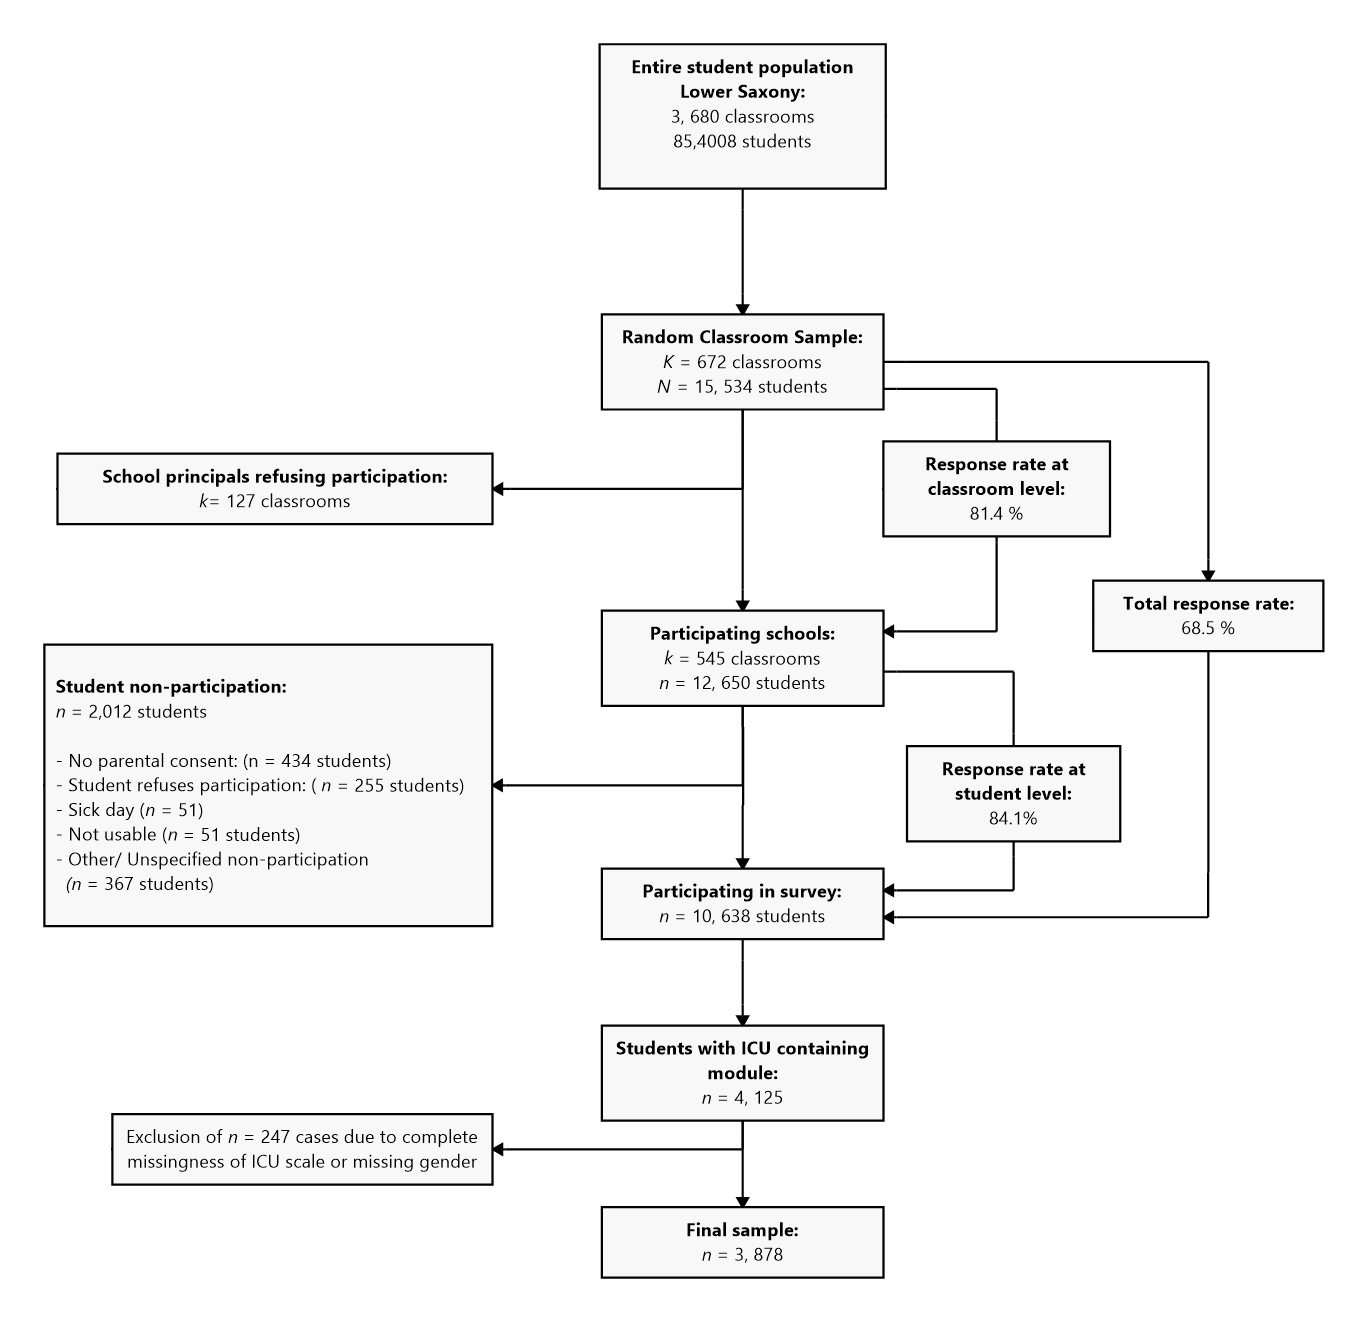
\includegraphics[width=\textwidth]{../figures/flowchart.png}
		\caption*{\textit{Note.} Figure adapted from \parencite{kliem_factor_2019}.}
	\end{figure}

The survey was modularized, i.e. there were different versions of the survey randomly assigned to the participants.
The ICU was only part of 1/3 of the distributed survey forms.
Accordingly, \textit{n} = 4,125 students received a survey version containing this scale.
The survey was approved by the federal school board of Lower Saxony (Nieders\"achsische Schukbeh\"orde) as well as the Ministry od Education of Lower Saxony (Nieders\"achsisches Kultusministerium).
Written parental consent was obtained for each student prior to student participation.
Students were informed, that their participation was entirely voluntary and anonymous.
Students could refuse participation independent of their parent's consent.
Students additionally had the option to skip individual questions.
Further details regarding the sampling procedure can be obtained from \parencite{bergmann_jugendliche_2017}

\subsubsection{Survey Setting}
The survey was conducted in the classroom setting during school time.
It was carried out by trained research assistants.
A research assistant as well as a teacher were present during the survey.
Their role was to ensure orderly conduct but not to interfere with the students filling in the forms.


\subsubsection{Sample Descriptives}
The final sample for the present analysis consisted of \textit{N} = $3878$ 9th grade students.
Students age ranged from $13$ to $19$ years with a mean age of \textit{M} = $14.88$ years (\textit{SD} = $0.71$).
The self-reported gender was $0.49$\% female (\textit{n} = $1992$  individuals) and $48.63$\% male (\textit{n} = $1886$ individuals).
Participants could not indicate a non-binary option.

\subsection{Measures}


\subsubsection{Callous-Unemotional Traits}
Callous-unemotional traits  were assessed using the German translation of the Inventory of callous unemotional traits \parencite{essau_callous-unemotional_2006}.
The scale comprises 24 self-report items rated on a 4-point Likert scale ranging from "Not at all true" (0) to "Definitely true" (3).
The internal consistency (Cronbach’s alpha) for the three subscales of the German version obtained in a similar sample are reported as: $\alpha = .64$ (unemotional),
$\alpha = .70$ (callousness) and $\alpha = .73$ (uncaring) \parencite{essau_callous-unemotional_2006}. 
A recent large Meta-Analysis by Cardinale and Marsh \parencite*{cardinale_reliability_2017} confirms acceptable reliability based on a pooled total sample of 27,947
subjects: $\alpha = .71$ (unemotional), $\alpha = .75$ (callousness) and $\alpha = .80$ (uncaring). 
These findings are in line with the Cronbach’s alphas found in the present sample:
$\alpha = .71$ (unemotional),  $\alpha = .72$ (callousness) and  $\alpha = .79$ (uncaring). \todo{check whether these alphas are actually correct}


\section{Data Analysis}
Data analysis was be conducted in the R statistical programming environment \parencite{R} (version 3.6.3). 
Further information regarding the computational environment as well as documentation of the corresponding analysis 
code can be obtained from appendix \todo{add reference to appendix}. 

\subsection{Data Processing and Cleaning}
Data was imported into R from SPSS. 
ICU items were recoded to comply with the intended original scaling.
They were furthermore inverted as intended and renamed. 
%The anti-social behavior items showed a large number of missing value as they were follow-up items to identically worded filter item asking whether the target behavior had ever been excibited.
%The missing values pertaining to the negation of the filter item where hence recoded to "never".  

\subsection{Missing Data Handling}
As the present dataset has been used for previous published research we will handle missing data in the same manner to obtain matching completed data.
The data was imputed using single imputation and predictive mean matching as implemented in the R package \texttt{mice}, \nptextcite{mice}).
All ICU items as well as age and gender was used to predict the missing values.
%The additional variables analyzed for the present study will be imputed in a similar manner, i.e. only the ICU items will be used for missing value prediction.
I have abstained from multiple imputation in the present study as I do not feel that the gain in precision justifies the added layer of complexity.
The focus of the present study is exploratory rather than confirmatory in nature and hence does not rely on point estimates and their corresponding standard error.

\subsection{Data Preparation for Network Analysis}
There are several recommendation of how to best prepare data for a network analysis. 
Especially regarding violations of multivariate-normality.
As the data was in clear violation of the normality assumption it was transformed using the non-paranormal transformation \parencite{liu_nonparanormal_2009}.
All items in the present analysis could be characterized as ordinal for which the use of polychoric correlations are recommended whenever analyses are based on correlation matrices.
Analyses comprising non-transformed correlations were also incorporated in the multi-verse. 
This corresponds to current findings indicating that the use of polychoric correlations could result in spurious negative edges \parencite{epskamp_estimating_2018}.
Epskamp and colleagues hence recommend comparing the results obtained using polychoric correlations to those obtained using Spearman correlations.  

Entering items with high topological overlap as nodes to the same network can be problematic.
The network edges represent partial correlations i.e.~associations between items taking into account all other items in the network.
Items with a high overlap will make it unlikely that there are any unique associations left to account for.
We hence searched for potential pairs of redundant nodes, that is nodes that are highly inter-correlated and that correlate to the same degree with other variables.  
This search was conducted by application of the Hittner method for comparing dependent correlations \parencite{hittner_monte_2003} as implemented in the \texttt{goldbricker()} function from the \texttt{networktools} package \parencite{networktools}.
This procedure did not indicate any considerable item overlap.

%\subsection{Statistical Analysis}

%Partial correlation networks were fit to a node sets comprising all 24 ICU items.
%I will refer to the analysis and results corresponding to this node set as "psychometric network" or "ICU network"

%Set (ii) comprises the aggregated ICU sub-scales \textit{"Lack of remorse or guilt"} (callous: \#2, \#5, \#9, \#13, \#16, \#18), 
%\textit{"Callous lack of empathy"}  (uncaring: \#4, \#8, \#12, \#17, \#21, \#24), 
%\textit{"Shallow or deficient affect"} (unemotional: \#1, \#6, \#10, \#14, \#19, \#22), 
%\textit{"Unconcerned about performance"} (careless: \#3, \#7, \#11, \#15, \#20, \#23) as well as measures of bullying behavior.
%The networks stemming from this node set will be evaluated from a psychological network perspective investigating the unique associations between nodes as well as the roles of certain nodes within the network. The specific parameters that will be interpreted for this purpose are outlined below.


\subsection{Descriptive Statistics}
Descriptives statistics were computed for all demographic variables.
Basic psychometric scale characteristics were computed for the ICU scale (item mean, item-rest correlations).
Correlations on subscale level are furthermore reported.


\subsection{Network Estimation}

Psychological network analysis is a fairly recent technique with a multitude of current methodological developments.
To incorporate the effects of several potentially applicable analytical decisions I conducted a multi-verse analysis \parencite{steegen_increasing_2016}. 
Table \ref{tab:decisions} contains an overview of the decisions and their corresponding options which are likely to be justifiable given the data at hand.

\begin{table}

\begin{ThreePartTable}
	\begin{TableNotes}
		\item \textit{Note.} 
		 \item MGM = Mixed Graphical Model ; GGM = Gaussian Graphical Model; EBIC~=~extended Bayesian information criterion; CV~=~cross-validation; RIC~=~rotation information criterion; StARS~=~stability approach to regularization selection.
	\end{TableNotes}
	\begin{longtabu} to \linewidth {
			X[4,l]
			X[4,l]
			X[4,l]}
		\caption{\label{tab:decisions}\protect\linebreak[1]
			\textit{Overview of defensible analytical decisions}} \\
		\toprule
		\multicolumn{1}{l}{Decisions} & \multicolumn{1}{l}{Options} & \multicolumn{1}{l}{References}\\
		\midrule
					Data transformation            & none; non-paranormal transformation    & \nptextcite{liu_nonparanormal_2009}          \\
					Network estimation             &                                        &  \\
					~~Correlation type               & Spearman, polychoric                    &  \nptextcite{epskamp_tutorial_2018}      \\
					~~Modeling approach              & Mixed Graphical Models (MGM),          &  \nptextcite{mgm}\\
					                               & Gaussian Graphical Models (GGM)        &  \nptextcite{epskamp_tutorial_2018}         \\
					~~Sparsity                       & Regularization                        &  \\
					                               & Correction for multiple testing        & \nptextcite{williams_nonregularized_2019}   \\
					~~Shrinkage tuning               & EBIC, CV, RIC, StARS                   & \nptextcite{wysocki_penalty_2019}          \\
					~~EBIC tuning parameter $\gamma$ & 0, 0.25, 0.5                           & \nptextcite{epskamp_tutorial_2018}         \\ 
		\bottomrule
\insertTableNotes 
\end{longtabu}
\end{ThreePartTable}
\end{table}

		The modeling decisions in table \ref{tab:decisions} above will be combined in as many ways as feasible.
		However, the current implementation of modeling techniques does not feasibly allow for a combination in a full-factorial way.
		Specifically, the default functions of the \texttt{bootnet} package  \parencite{epskamp_estimating_2018} will be used with every reasonable parameter constellation.
		Figure \ref{fig:multiverse} provides an overview of the implementation of the analytical decisions outlined above. 

	\begin{figure}[H]
		\caption{\label{fig:multiverse}\protect\linebreak[1] 
			Overview of implemented modeling techniques}
		\centering
		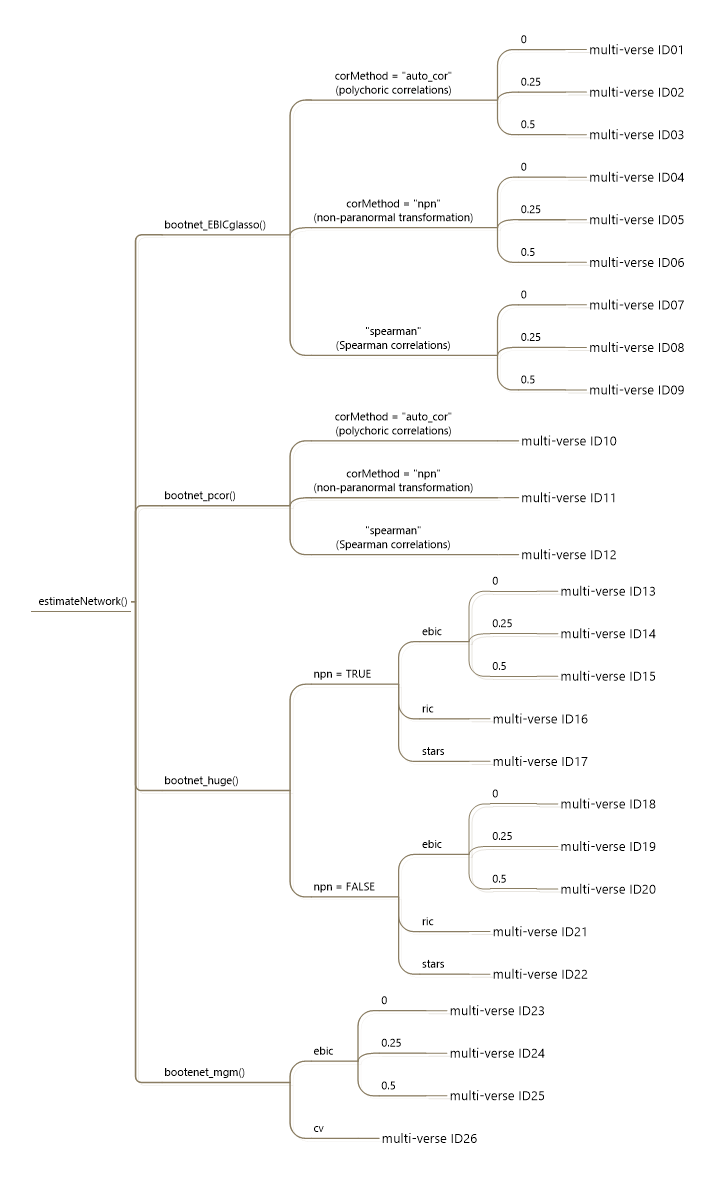
\includegraphics[width=\linewidth]{../figures/multiverse.png}
	%	\caption*{\textit{Note.} ICU = Inventory of Callous-Unemotional Traits.}
	\end{figure}

		We will now  provide a detailed justification of each step in the analysis process explaining the necessary decisions to be made as well as the options available:

		\paragraph{Data Transformation}
		Epskamp \parencite*{epskamp_estimating_2018} recommends normalizing variables with a skewed distributions using the non-paranormal transformation \parencite{liu_nonparanormal_2009}.
		As there are currently no clear guidelines regarding this transformation we will repeat each of the analyses with untransformed variables. %check that

\paragraph{Modeling Approach}
		The networks can be modeled using either a \gls{ggm}  or \gls{mgm}.
		GGMs assumes Gaussian data i.e. following a normal distribution.
		However, given the nature of the variables investigated in the present study such distributions seem unlikely for several nodes.
		MGMs takes the ordinal nature of the data into account by estimating the node edges using exponential mixed graphical model as introduced by Yang and colleagues \parencite*{yang_mixed_2014}. 
		As part of the multi-verse approach have incorporated both modeling techniques as the 4-point scale underlying the ICU represents the idea of a continuous variable.

		\paragraph{Network Sparsity} To avoid the estimation of spurious edges and thereby overfitting the network to the data and increase the risk of false positives, network edges are often estimated using regularization.
		Regularization shrinks edges and sets small edges to zero, producing a sparse and parsimonious model.
		For the estimation of GGM the application of the graphical LASSO (GLASSO) is frequently recommended (a variant of the LASSO applicable to a correlation matrix).
		Tuning of the shrinkage is commonly achieved choosing the model with the lowest  \gls{ebic}.
		This approach is implemented in the \texttt{qgraph} package \parencite{epskamp_qgraph_2012}.
		The EBIC itself relies on a tuning parameter $\gamma$.
		This tuning parameter influences the trade-off between including false-positive edges and removing true edges.
		The hyperparameter $\gamma$ is usually set between zero and 0.5 \parencite{epskamp_tutorial_2018} with 0.5 being the most frequently chosen setting.
		With a $\gamma$ closer to 0.5, the EBIC will favor a simpler model containing fewer edges.
		Consequently with a $\gamma$ near zero, the more the EBIC will favor a model with more edges.
		I have incorporated $\gamma$'s of 0, 0.25 and 0.5 as part of the present multi-verse analysis.

		However, there is recent methodological work indicating that the EBIC might not be the ideal information criterion for tuning the shrinkage parameter \parencite{wysocki_penalty_2019}.
		The multi-verse analysis will hence also incorporate alternative methods (i.e. gls{ric}, gls{star}) for determining optimal regularization.
		These alternative approaches to selecting the shrinkage parameter for a GGM are implemented in the \texttt{huge} package \parencite{huge}.
		The MGM estimation as implemented in the \texttt{mgm} package \parencite{mgm} regularizes the estimated edges via a LASSO penalty.
		Here tuning of the penalization can be achieved via EBIC or \gls{cv}.

		Recent debate \parencite{williams_nonregularized_2019} questions the general need for regularization and argues that these techniques might only be justifiable when in deed a sparse network can be assumed to underly the data.
		Hence following recent recommendations by Williams and colleagues \parencite{williams_nonregularized_2019} we will also estimate network models without regularization, albeit still controlling for the false-positive rate.

		\subsection{Psychometric Network}

		\paragraph{Edge Estimation}
		For all primary analyses we will estimate the stability of edges with bootstrapped confidence intervals using the \texttt{bootnet} package \parencite{epskamp_estimating_2018}.
		The number of bootstrap samples for this and all other bootstrap procedures will be determined by computational feasibility.

		\paragraph{Node Statistics}
		Node centrality measures (\textit{betweenness centrality}, \textit{closeness centrality} and \textit{node strength}) are traditionally interpreted as the relative influence of a node in the network.
		More recently the interpretability of closeness centrality and betweenness centrality have been questioned and their use discouraged.
		Node strength, (which is the sum of all weighted edges of a given node) however, has been found to be akin to factor loadings.
		It hence offers information whether an item may belong to multiple latent dimensions.
		The \textit{expected influence centrality} recently suggested by \textcites{robinaugh_identifying_2016} overcomes some of the shortcomings of other centrality measures and has been found to be strongly associated with observed node influence. 
		It is computed in the same manner as node strength however maintaining the edge sign. It is hence especially useful in networks where negative edges are present.
		I have hence computed both node strength as well as node expected influence, both as implementen in the \texttt{bootnet} package \parencite{epskamp_estimating_2018}.
		
		\paragraph{Community Detection}
		A community detection algorithms was applied to all estimated adjacency matrices from the multi-verse.  The walktrap algorithm as implemented in the \texttt{igraph} package was used for this \parencite{igraph}. As community detection does not provide point estimates but items sets, this analysis was not bootstrapped for lack of pooling method of such a procedure.
		
		\paragraph{Bridge Nodes and Within Community Centrality}
		I also identified important nodes that may serve as bridges between the communities by computing the \textit{bridge expected influence index} via the \texttt{bridge()} function of the \texttt{networktools} package \parencite{networktools}.
		Bridge expected influence is the sum of the edge weights connecting a given node to all nodes in the other community or communities \parencite{jones_bridge_2019}.
		Following the suggestions of Blanken and colleagues \parencite*{blanken_role_2018} I additionally analyses the edge weights a given node has within its community (\textit{stabilizing index}). I used the four factors corresponding to the LPE specifier for this analysis. The stabilizing index is not currently implemented in any network analysis package and was hence computed via a custom function.


%		\subsection{Psychological Network Analysis of CU-Traits Facets and Anti-Social Behavior}
%		The psychological network analysis comprising the second node set, as outlines above, will compute the same network statistics as outlined for the psychometric analysis apart from any estimates regarding the detection or centrality of communities.
%
%		\subsection{Stability and Robustness of Estimates}
%		We will evaluate the stability of the node metrics by implementing a subset bootstrap procedure as implemented in the \texttt{bootnet} package \parencite{epskamp_estimating_2018}.
%		We will also calculate the \textit{centrality stability correlation coefficient} (CS-coefficient) which represents the maximum proportion of participants that can be dropped while maintaining 95\% probability that the correlation between centrality metrics from the full data set and the subset data are at least .70.






%4. Ergebnisse. In diesem Teil werden die Ergebnisse Ihrer Untersuchung 
%dargestellt und mit Blick auf die Fragestellung ausgewertet. 
%Gliedern Sie den 
%Ergebnisteil anhand Ihrer Fragestellungen bzw. Hypothesen und machen Sie diese 
%Gliederung durch Überschriften deutlich. 
%Beginnen Sie mit der Darstellung der 
%deskriptiven Statistiken (z. B. Mittelwerte und Standardabweichungen, Korrelationen 
%zwischen den untersuchten Variablen). 

%Anschließend berichten Sie die Ergebnisse zu 
%Ihren Fragestellungen und Hypothesen. Beschreiben Sie detailliert Ihre Datenanalysen 
%und Ihre Ergebnisse. 
%Ziehen Sie ein kurzes Fazit hinsichtlich der Ablehnung oder 
%Beibehaltung der Hypothese, achten Sie aber darauf, dass Sie Ihre Ergebnisse hier 
%lediglich beschreiben, ohne sie zu interpretieren und Schlussfolgerungen daraus zu 
%ziehen! 

%Beschreiben Sie die Ergebnisse in der Vergangenheitsform. 
%Präsentieren Sie Ihre Ergebnisse auch tabellarisch und graphisch. 
%Achten Sie darauf, dass Sie Tabellen 
%und Abbildungen nicht überladen. Achten Sie auch darauf, Tabellen und Abbildungen 
%korrekt zu beschriften. 
%Die Formatvorschriften für das Berichten statistischer 
%Kennwerte, zur Ergebnisdarstellung und zur Formatierung von Tabellen und 
%Abbildungen entnehmen Sie den aktuellen APA-Standards. 

% Aus dem Bewertungsschema
% Ergebnisteil ist in Bezug auf die Fragestellungen/Hypothesen sinnvoll gegliedert.
% Relevante vorgeschaltete Analysen werden berichtet (z. B. deskriptive Statistiken).
% Die Auswertungsverfahren werden benannt und korrekt angewendet. 
% Es werden Ergebnisse der Verfahren beschrieben, die für die Hypothesentests relevant sind. 
% Die Ergebnisse werden anhand der statistischen Kennwerte richtig und gut nachvollziehbar dargestellt.    
% Die Ergebnisse werden in Bezug zu den Hypothesen gesetzt. 
% Es wird bei der Darstellung der Ergebnisse angemessener Gebrauch von aussagekräftigen Tabellen und Abbildungen gemacht. 

%\section{\thesection. Section Title}
%\subsection{\thesubsection. Subsection title}
%\subsubsection{\thesubsubsection. Subsubsection title}

% !Rnw root = 00_main.Rnw
 
\section{Results}

The following section will present the results from the present analyses.
After an overview of general descriptive statistics the results pertaining to each 
network analysis are presented separately albeit following a fairly parallel structure.


\subsection{Missing Data Analysis}
Figure \ref{fig:itemwise_missingness} shows the item wise missingness for all variables. 
Apparent patterns of sequentially missing items (i.e. ICU \#1 to ICU\#10 and ICU\#11 to ICU\#24) largely correspond to
pages of the questionnaire indicating these are instances of pages having been (accidentally) skipped.
Item wise missingness ranged from 0.016\% (battery teacher) to 10.39\% (ICU \#19) with a mean of 2.03\% (\textit{SD} = 1.75\%).
\begin{figure}[h!]
	\caption{\label{fig:itemwise_missingness}\protect\linebreak[1]\textit{Item wise missingness}}
	\centering
	\includegraphics[width=\linewidth, trim = {0.5cm 0cm 0cm 0mm}, clip]{../figures/missingness.pdf}
	\caption*{\textit{Note.} ICU = Inventory of Callous-Unemotional Traits.}
\end{figure}


\subsection{Descriptive Statistics}
Table \ref{tab:descriptives} \todo{add table} presents the descriptive statistics on scale level for all scales assessed in the present analyses.
All descriptives were computed using the imputed data set.

	\begin{ThreePartTable}
		\begin{TableNotes}
			\item \textit{Note.} 
			\item (-) indicates inversely scored items.
		\end{TableNotes}
		\begin{longtabu} to \linewidth {>{\raggedright}X>{\centering}X>{\centering}X>{\centering}X>{\centering}X>{\centering}X>{\centering}X}
			\caption{\label{tab:icu_itemcharacteristics}\protect\linebreak[1]
				\textit{Item characteristics for ICU items}}\\
			\toprule
			\multicolumn{1}{c}{Item} & \multicolumn{1}{c}{\textit{M}} & \multicolumn{1}{c}{\textit{SD}} & \multicolumn{1}{c}{\textit{Skew}} & \multicolumn{1}{c}{Kurtosis} & \multicolumn{1}{c}{\textit{SE}} & \multicolumn{1}{c}{$r_{it}$}\\
			\midrule
			1 (-) & 1.94 & 0.88 & -0.47 & -0.54 & 0.01 & 0.36\\
			2 & 1.22 & 0.88 & 0.45 & -0.41 & 0.01 & 0.10\\
			3 (-) & 0.83 & 0.89 & 0.86 & -0.09 & 0.01 & 0.42\\
			4 & 0.27 & 0.63 & 2.60 & 6.56 & 0.01 & 0.38\\
			5 (-) & 1.10 & 1.03 & 0.46 & -1.00 & 0.02 & 0.44\\
			\addlinespace
			6 & 1.38 & 1.04 & 0.24 & -1.10 & 0.02 & 0.38\\
			7 & 0.48 & 0.79 & 1.67 & 2.10 & 0.01 & 0.35\\
			8 (-)& 0.96 & 0.89 & 0.63 & -0.37 & 0.01 & 0.50\\
			9 & 0.70 & 0.85 & 1.03 & 0.21 & 0.01 & 0.38\\
			10 & 1.30 & 0.95 & 0.32 & -0.80 & 0.02 & 0.18\\
			\addlinespace
			11 & 0.47 & 0.71 & 1.48 & 1.73 & 0.01 & 0.38\\
			12 & 0.73 & 0.88 & 1.07 & 0.30 & 0.01 & 0.44\\
			13 (-) & 1.71 & 0.88 & -0.18 & -0.70 & 0.01 & 0.14\\
			14 (-) & 1.91 & 0.88 & -0.44 & -0.53 & 0.01 & 0.32\\
			15 (-) & 0.79 & 0.82 & 0.82 & 0.06 & 0.01 & 0.45\\
			\addlinespace
			16 (-) & 0.70 & 0.86 & 1.04 & 0.22 & 0.01 & 0.56\\
			17 (-) & 0.78 & 0.87 & 0.89 & -0.02 & 0.01 & 0.55\\
			18 & 0.81 & 0.94 & 0.92 & -0.20 & 0.02 & 0.28\\
			19 (-) & 1.99 & 0.89 & -0.52 & -0.55 & 0.01 & 0.23\\
			20 & 0.85 & 0.86 & 0.74 & -0.22 & 0.01 & 0.26\\
			\addlinespace
			21 & 0.42 & 0.75 & 1.85 & 2.80 & 0.01 & 0.49\\
			22 & 1.30 & 1.01 & 0.37 & -0.94 & 0.02 & 0.33\\
			23 (-) & 1.01 & 0.84 & 0.49 & -0.41 & 0.01 & 0.43\\
			24 (-) & 1.28 & 0.87 & 0.21 & -0.64 & 0.01 & 0.39\\
			\bottomrule
			\insertTableNotes
		\end{longtabu}
	\end{ThreePartTable}


\paragraph{Scale and Item Characteristics}
Table \ref{tab:icu_itemcharacteristics} \todo{add table} presents scale and item characteristics for the ICU. 
Pairwise correlations of all constructs assessed in the present analysis are given in table  \todo{add table reference and table}.  

\subsection{Estimation Problems}
Some models from the multi-verse were not estimable with the current implementation of the \texttt{bootnet} package.
For the lack of informative error messages the nature of the estimation problems is unknown.
This concerns multi-verse ID's 21 and 22 for both the psychometric network analysis as well as the psychological network analysis.
Since the regularization techniques in both of these estimators rely on resampling it is possible that the low prevalence of some items led to 
zeros which caused the estimation to stop. Other possibilities (at least for the psychological network) might be the estimation of an empty graph i.e. 
the estimation of all edges to equal zero.
The final multi-verse hence comprised 24 different estimation procedures.
  
\subsection{Psychometric Network Analysis}

\subsubsection{Network Description}
There was no topological overlap detected for the ICU items. 
Correspondingly the psychological network analysis included all 24 ICU items as nodes. 
With 24 nodes in the network the number of possible edges was 300 as $\frac{24 * 25}{2} =300$.
The number of non-zero estimated edges ranged from $153$ (51\%) (name of analysis). to $276$ (92\%) (name of analysis) \todo{add names of analyses}.
Mean number of edges was $198.96$ (\textit{SD} = $35.09$.
The number of negative edges ranged from $26$ to $107$ with a mean of $51.35$ (SD = $22.05$. \todo{add percentages}
None of the analyses resulted in isolated nodes (i.e. nodes that are not connected to any other node in the network).

\subsubsection{Network Structure}


\paragraph{Edge Weights}

Figure \ref{fig:icu_net} shows the network model graph featuring the median edge weights over all implemented estimation models.
Graphs for each individual network from the multi-verse analysis can be found in appendix \todo{add reference to appendix}.
Edge width is proportional to the maximum edge which was ... \todo{add edge statistics}
When interpreting the size of the edge weights it has to be taken into account that partial correlations are usually smaller than
first-order correlations.

\begin{figure}[H]
	\caption{\label{fig:icu_net}\protect\linebreak[1]\textit{Medium ICU Network of all Implemented Estimators}}
	\centering
	\includegraphics[width=\linewidth]{../figures/ICU_network.pdf}
	\caption*{\textit{Note.} Node numbers correspond to ICU item numbers. Colors correspond to subscale membership of the corresponding items.
	Blue indicates positive edges, red negative ones.}
\end{figure}

\subsubsection{Node Centrality}
Figure \ref{fig:icu_node_indices} presents the node expected influence centrality as well as node strength for all nodes in the ICU network.

As for the edge weights the histograms correspond to the bootstrap analyses whereas the points correspond to the point estimates per analysis.

\begin{figure}[H]
	\caption{\label{fig:icu_node_indices}\protect\linebreak[1]\textit{ICU Local Node Centrality Indices}}
	\centering
	\includegraphics[width=\linewidth]{../figures/node_centrality_icu.pdf}
	\caption*{\textit{Note.} ICU = Inventory of callous-unemotional traits. Points correspond to medium over all estimated models. Error bars correspond to 2 * medium SD obtained from the bootstrap samples.}
\end{figure}


\paragraph{Community Indices}
Figure \ref{fig:meso_plot} depicts the meso-level node indices bridge expected influence and the stabilizing index. 

\begin{figure}[H]
	\caption{\label{fig:meso_plot}\protect\linebreak[1]\textit{ICU Meso-Level Node Centrality Indices}}
	\centering
	\includegraphics[width=\linewidth]{../figures/meso_plot.pdf}
	\caption*{\textit{Note.} ICU = Inventory of callous-unemotional traits. Points correspond to medium over all estimated models. Error bars correspond to 2 * medium SD obtained from the bootstrap samples.}
\end{figure}

\subsubsection{Dimensionality}
\paragraph{Community detection}
Figure \ref{fig:communities} depicts the detected communities per implemented estimation model.
In 13 of the 23 different estimation implementations the walktrap algorithm detected two communities.
These two communities correspond to the sets of positively (\#2, \#4, \#6, \#7, \#9, \#10, \#11, \#12, \#18, \#20, \#21, \#22 ) and negatively (\#1, \#3, \#5, \#8, \#13, \#14, \#15, \#16, \#17, \#19, \#23, \#24) scored items.
In six cases, three communities were detected. 
These correspond to the set of positively worded items, as well as the items sets (\#1, \#13, \#14, \#19) and (\#3, \#5, \#8, \#15, \#16, \#17, \#23, \#24).    
The remaining three estimations detected 5 or 6 communities.

\begin{figure}[H]
	\caption{\label{fig:communities}\protect\linebreak[1]\textit{Detected communities (walktrap) for each different network estimation}}
	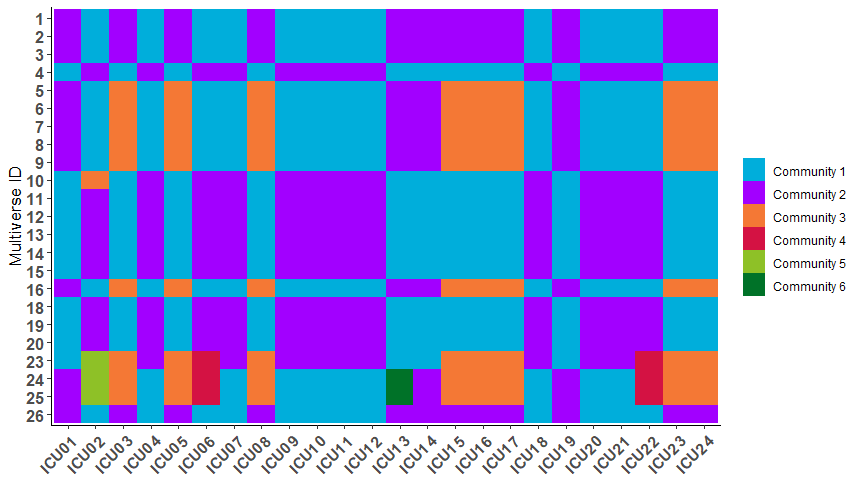
\includegraphics[width=0.9\linewidth]{../figures/communities.png}
	\caption*{\textit{Note.} ICU = Inventory of Callous-Unemotional traits.}
\end{figure}


%\subsection{Psychological network analysis}
%\subsubsection{Network description}
%
%The \texttt{goldbricker()} function indicated topological overlap of the items "I ridiculed a teacher in front of other students." and 
%"I was very mean to a teacher.". 
%These items were hence combined to one node (by averaging).
%
%Correspondingly the psychological network analysis comprised 12 nodes (4 ICU facets and 8 indicators of anti-social behavior). 
%With 12 nodes in the network the number of possible edges was 78 as $\frac{12 * 13}{2} =78$.
%The number of non-zero estimated edges ranged from  (\%) (name of analysis). to  (\%) (name of analysis) \todo{add names of analyses}.
%Mean number of edges was  (\textit{SD} = .
%The number of negative edges ranged from  to  with a mean of (SD = . \todo{add percentages}
%None of the analyses resulted in isolated nodes (i.e. nodes that are not connected to any other node in the network).


% Example figure to copy & paste

%\begin{figure}[h!]
%	\caption{\label{fig:}\protect\linebreak[1]\textit{s}}
%	\centering
%	\includegraphics[width=\linewidth]{../figures/.pdf}
%	\caption*{\textit{Note.} ICU = Inventory of Callous-Unemotional Traits.}
%\end{figure}
%5. Diskussion. Nennen Sie die Zielsetzung Ihrer Arbeit und fassen Sie 
%zunächst die wichtigsten Ergebnisse in Bezug auf Ihre Hypothesen in einem (oder 
%wenigen) Absatz/Absätzen zusammen. Nennen Sie dann Ihre Schlussfolgerungen 
%(Ihre Interpretation der Ergebnisse) und begründen Sie diese. Zitieren Sie hier auch 
%noch einmal die wichtigen Arbeiten, auf die Sie sich stützen und die helfen, die 
%Ergebnisse zu verstehen. 
%Diskutieren Sie, wenn möglich, auch alternative Erklärungen und legen Sie dar, 
%was für Ihre Interpretation der Ergebnisse spricht. Gehen Sie auch ausführlich auf die 
%inhaltlichen und methodischen Grenzen Ihrer Untersuchung ein und beschreiben Sie, 
%welche Anschlussfragestellungen und weiteren Forschungsbedarfe sich aus Ihrer 
%Studie ergeben. Reflektieren Sie abschließend auch theoretische und praktische 
%Implikationen Ihrer Arbeit. 


% Aus dem Bewertungsschema:
% Ergebnisse werden im Hinblick auf Hypothesen und Fragestellung angemessen zusammengefasst. 
% Es werden alle Untersuchungsfragen beantwortet. 
% Die Ergebnisse werden aus theoretischer Perspektive interpretiert.  
% Es wird deutlich aufgeführt, was für die eigene Interpretation der Befunde spricht.
% Alternative Interpretationsmöglichkeiten werden diskutiert. 
% Die Ergebnisse werden aus methodischer Perspektive interpretiert. 
% Potentielle Einschränkungen der Untersuchung und des eigenen Vorgehens werden benannt und ihre Konsequenzen für die % Interpretation diskutiert. 

% Theoretische und praktische Implikationen werden abgeleitet. 
% Die praktische Relevanz wird verdeutlicht. 
% Weiterer Forschungsbedarf und Ideen für zukünftige Forschung werden beschrieben. 

%\section{\thesection. Section Title}
%\subsection{\thesubsection. Subsection title}
%\subsubsection{\thesubsubsection. Subsubsection title}
%\paragraph{\theparagraph. Paragraph title}%\section{\thesection. Section Title}
%\subsection{\thesubsection. Subsection title}
%\subsubsection{\thesubsubsection. Subsubsection title}
%\paragraph{\theparagraph. Paragraph title}

\section{Discussion}
The aim of the present was twofold. 
First, to provide a psychometric analysis of the ICU from a network perspective and compare and contrast the results obtained to existing research.
Second, to apply network analyses techniques to extend current knowledge regarding the role of the LPE specifiers with respect to 
various form of anti social behavior. ICU correlates (intimate partner violence, ....)
The second aim could unfortunately not be implemented as intended due to insufficient variability in the dataset at hand.
The following section will hence discuss the results from the psychometric network analysis.

\subsection{Influence of modeling decisions - Multi-verse approach}
The point estimates obtained implementing the various modeling decisions varied considerably.
However, the approach of this study was exploratory in nature (as opposed to predictive or explanatory). 
Consequently, my interpretation will not rely too heavily on point estimates.
Combining the various point estimates as well as boot strapped confidence interval allows to distill the results into general tendencies.
These seem to be quite robust across individual modeling choices and will hence be the focus of result interpretation.  

\subsection{Psychometric network of ICU items}
Regarding the first aim, several findings from the psychometric literature could be replicated.
Method factors could also e found with the spinglas algorithm detecting a community of nodes that represented all positively worded items.
Some evidence for content factors was also found with one community consisting entirely of nodes that correspond to items from the "careless" subscale.
The comparably high missingness of item \#19 ("I am very expressive and emotional (-)") which, with 10.39\% missing cases, was on average more than five times as often as the other items suggests 
missingness that is not merely attributable to occasional sloppy answering style.
A closer look at the German translation (\textit{"Ich bin sehr extrovertiert und gefühlsbetont."})[sic!] suggest that the missingness might be attributable to
students not being familiar with the term "extrovertiert" (which should actually be "extravertiert", a common mistake that 9th grade students are likely unaware of).
Should this be the case, missingness for this item might not be at random as it might be related to factors such as verbal intelligence or parental education.

\subsubsection{Network edges}
Most estimated networks were rather dense.
This is likely due to the fact that the scale consists of a large number of highly similar items.
A closer look at the network edges suggests that a large number of strong edges are likely due to similarity in item wording. 
In the German translation the item wordings of some items are more alike compared to the English original.
Items \#1, \#6 and \#22 have very similar item wording and are arguably semantically closer compared to the English original.
Both feelings and emotions are translated with the German word "Gefühle". 
It might be argued, that adolescents might not be aware of the subtle differences of these two concepts, yet the primary 
... of the German items suggests the physical expression of emotionality is referred to while the original English items could also cover the verbal expression of inner states.
Similarly the item pair \#8 and \#21 are arguably semantically closer in the German translation that in the English original. 
"Concerned" and "unimportant" are translated with "wichtig" and "unwichtig" resulting in the two items almost reading as exact opposites of one another.
The strong relationship of item \#16 and \#17 might be a combination of similar wording (both contain "hurt"), carryover due to their location as well as both od them being positively worded.
The combination of these three features might explain the strong relationship. While \#16 is intended to tap into the callous domain it might have captured more of the uncaring domain in this context.
This might also have been enhanced by the German translation reading "Wenn ich jemanden verletzt habe, entschuldige ich mich" vs the English original "I apologize ("say I am sorry") to persons I hurt."
The focus of the German translation is arguably shifted away from the callous habit of (not) apologizing towards an reaction to having hurt someone (i.e. an act of caring).
The opposite, i.e. more semantic distance to other items of the domain can be observed for item \#12. The English "uncaring" has been translated with "gleichgültig" (indifferent). 
In combination with "kalt" (cold) item \#12 reads as if it refers to emotional expressions rather than behavior which might explain its closeness to items from the unemotional domain in the network.

Most edges are positive (as would be expected) however, some negative edges can be observed.
While most of these negative edges are very small and can likely be ignored two patterns seem to emerge.
First, the highest number of negative edges are connected to nodes belonging to the "unemotional" dimension.
The unemotional dimension of the ICU has received considerable criticism as being to focused on lack of emotional expression rather than ... \todo{continue arguments}
researchers argued that these kinds of items might tap into unrelated constructs such as conditions on the autism spectrum (ASD) or mood disorders \todo{add reference}.
As the prevalence of ASD and mood disorders is likely higher than psychopathy in the present at hand some of the negative edges could possibly be explained by this reasoning.
Furthermore the items \#2, \#10, and \#13 which have previously been criticized for their poor psychometric properties have a high number of negative edges providing further evidence of them not measuring the intended construct. 

\subsubsection{Node centrality}
The amount of negative edges is also depicted when comparing the node strength to the node expected influence. 
While the former represents the sum of absolute edges for a given node, the latter takes the edge sign into account and subtracts negative edges. 
Nodes for which node strength and node expected influence differ considerably are those with more or stronger negative edges.
As stated in the previous paragraph, nodes corresponding to items on the "unemotional" subscales are associated with a large amount of negative edges, with one noteworthy exception.
Item \#6 "I do not show my emotions to others" is among the most influential in the network.
Node centrality can be interpreted in various ways, from a more traditional latent variable perspective it is comparable to factor loadings. 
Indeed the most central nodes in the present analysis do correspond to those with the highest factor loadings presented in a recent paper based on the same dataset
\parencite{kliem_factor_2019}.
From a network theory perspective central nodes excert a greater influence on the entire system. 
These nodes might stabilize and "communicate" through their high number and or strong connections to other nodes.
This logic might be exemplified by node \#21 "The feelings of others are unimportant to me", 
not endorsing this will consequently lead to being concerned about other peoples feelings \#8,
and hence doing things to make them feel good \#24,
and not trying to hurt other's feelings \#17 which in turn will lead to apologizing should one have hurt someone \#16.
Item \#16 is a nice example of an item potentially undesirable in a latent variable context. 
An apology can be an expression of guilt and/or an expression of care. 
It can hence be expected to exhibit cross-loadings on the uncaring subscale \parencite{essau_callous-unemotional_2006}.
While cross-loadings are a  nuisance and threaten the "purity" of the latent construct they are potentially valuable from a network perspective as they potentially explain how the different symptoms are related
and information might "spread" through the network. 
Such nodes might furthermore prove useful as potential targets for interventions.

This idea is developed further in the centrality indices on a meso-level.
On the community level nodes with a high number of edges within the cluster are interpreted as stabilizing this facet whereas nodes with a high number of connections to other communities are termed
bridges \parencite{robinaugh_identifying_2016} or communicating symptoms \parencite{blanken_role_2018}.

From visual edge inspection it can be seen that the "unemotional" dimension as well as the "uncaring" dimension have a high number of strong within factor edges.
This ....\todo{add results from community analysis}.

These interpretation show that the theoretically assumed factor structure might by justified but very closely tied to fine semantic nuances that are not sustainable in translation. 
They might further be influenced by item order and coding.
  
 
\subsubsection{Dimensionality}
Two dominant communality patterns emerged.
The community structure that was uncovered most frequently was a 2-community solution with all positively worded items in one community and all negatively worded items in a second.
This is in line with multiple previous findings who discuss a strong influence of item wording on the factor structure of the ICU.

%\subsection{Psychological network analysis}
%
%\subsubsection{Network edges}
%Due to the low prevalence of the anti-social behavior items a large number of boot strapped samples resulted in non-positive definite correlation matrices.
%This was likely due to the fact that some of the bootstrap samples might not have contained any participants exhibiting the behavior in question.
%
%Whereas the psychometric networks containing only the ICU items were very stable across the estimation methods. This is not the case for the psychological networks.
%There were two major network structures emerging. One with the ICU factors where isolated from the behavioral items and a second where they were connected.
%
%A lack of connection of the CU-trait nodes with the indicators of anti-social behavior indicates that there was no unique variance between any these of these nodes.
%There are several potential explanations for this observation. 
%One is a general lack of variability - what does not vary also cannot co-vary. 
%A second possibility is a great topological overlap of the behavioral items and/or the ICU facets.
%The string connections within the behavioral items as well as within the ICU facets suggest this interpretation. 
%In addition the common method variance of the ICU facets and the behavior items correspondingly might account for a large share of variance. 
%
%However, within both the unconnected models as well as the connected solutions the estimated edges were very consistent. 
%For both the unconnected as well as the connected networks it was evident that the "unemotional" subscale was the most isolated one. 
%Its only week connection to the rest of the ICU subscales was consistently the "uncaring" factor. 
%This is in line with previous research indicating that the "unemotional" subscale shows the lowest correlation wit th ICU as a whole as well as with external criteria that the ICU is generally predictive of \parencite{cardinale_reliability_2017}
%In the connected network the connection between the ICU subscales and the behavioral items is consistently via the "callousness". 
%The strongest edge thereby being the "callousness" subscale and the extortion item.
%This as well is in line with previous research indicating that the callousness subscale shows the strongest associations with anti-social behavior.
%
%Accounting for the anti-social behavior the ICU facets did not constitute a latent factor in the sense that the network comprising the four CU-trait nodes was not fully connected.
%The unemotional and the careless facet where not connected in any of the estimations of the multi-verse. 
%The edge of the unemotional and the callousness facet was consistently weak. 
%The other three facets (uncaring, careless and callousness) consistently formed a cluster across all estimations. 
%
%These results are problematic with regard to the LPE specifier requiring two of the four facets to be present.
%The present analysis suggests that those facets are not equivalent, both in their internal organization as well as their relationship to behavioral covariates.
%While the uncaring facet is central with regards to within construct relationships and hence potentially important for the stability of the symptom network, 
%it is the callousness facet that showed unique associations with the anti-social behavior nodes. 
%
%
%Another noteworthy consistency among the estimated networks is that with the exception of the extortion item all other edges of the "callousness" facet with the behavioral items are negative.
%There are three possible explanations for this observation.
%(1) This could be indicative of a suppressor effect.
%(2) All networks which show the negative edges are based on polychoric correlations. 
%Polychoric correlations are known to cause spurious negative correlations in case there are too few observations in cross-tables. 
%Given the low prevalence of some of the items this is certainly a possibility in the data at had. 
%Due to this known weakness it is recommended to always compare networks based on polychoric correlations to their counterpart based on Spearman correlations \parencite{epskamp_tutorial_2018}.
%(3) 
%



%The high number of negative edges in the estimated networks is very evident. 
%\subsubsection{Node indices}


\subsection{Limitations}
The present study suffers from a several important limitations.
In this paragraph I will discuss these limitations pertaining to measurement concerns,
the sample population, methodological issues as well as theoretical shortcomings 

\subsubsection{Measurement related limitations}
First, the data only stems from self-report. 
Additional versions of the ICU are available (parent report and teacher report).
Findings should hence be compared to those obtained by other report. 
Furthermore, the ICU comprised question 873 to question 897 of a 901 item long survey form.
This location at the end of the questionnaire might have caused additional measurement error and facilitated the emergence of method artifacts in the form of common method variance.
The comparably high amount of missingness (see \ref{fig:missingness}) supports this possibility.
%Common method variance could be responsible could be responsible for some observed edges. 
However, most of common method variance (unless unique to a pair of items) should be excluded by the use of partial correlations.

The present study is a secondary analysis of existing data. 
The data were not collected with the present study in mind. 
Hence the questionnaires analyzed in the present study might not ideally capture the intended constructs.
Future studies employing network methodology should aim for measures that are tailored for use in a network analysis as well as in combination with the ICU.
Longitudinal...

The items assessing anti-social behavior were all school based. 
This had the obvious advantage that their wording was close to the everyday experiences of the participants and these items hence showed reasonable prevalence for the present analysis.
An obvious drawback is, that showing some of the more extreme behaviors (such as hitting a teacher) makes it likely to get expelled from school and hence not participate in the survey.
It can hence be expected that there might me a slight selection bias with respect to the top end of the scale.


\subsubsection{Limitations regarding Sample Population and Study Design}

The age range of the present sample was rather narrow due to the participants all attending the same grade.
While this provides a potentially more complete picture of that very age group it might limit generalizability of results.
The narrow age range might have provided additional challenges given the general low variability of the data at hand.

The data analyzed in the present study is cross-sectional, hence no causal conclusions are possible. 
While network theory highly relies on processes and interacting systems, the analysis of cross-sectional data for the generation of hypotheses is common. 
The exploratory insights obtained in the present study will nevertheless have to be replicated and confirmed in longitudinal designs.
It has to be furthermore reiterated, that the observed between-person effects should not be confused with within-person effects.

The assessment of pathology in a general population sample is a common practice. 
Conclusions that can be inferred about the population with high scores on the trait of interest, however, are limited.
Yet, the opposite also holds. Conclusions from a population characterized by features that are highly related to the trait under investigation likely suffer from collider bias. 
Future studies should ideally focus on a selection of participants that is independent of the variables in the model, yet at the same exhibit enough variability on the constructs of interest. 
In the context if network models careful phrasing of distinct items, that are meaningful yet similarly interpreted for a broad range of populations could help in this endeavor.
A focus solely on children who already have CD could limit advances in our understanding of how CD develops (Frick et al. 2014) \parencite{frick_can_2014}

\subsubsection{Methodological Limitations}
	- warn 

From <https://link.springer.com/article/10.1007/s00127-016-1319-z> 
- Suppressor effects (Lahey 2014)\parencite{lahey_what_2014}
Possibility of circularity (lahey 2014) 
 
 Differential variability \parencite{terluin_differences_2016}
 Nodes showing large differences in variance.
 
  Finally, network analysis is a rather recent technique. 
 Hence, methodology is still under development and best-practice recommendations regularly changing.
 The R package \texttt{bootnet} which was used for most of the present analyses for example was updated xz times
 during the preparation of the manuscript at hand. 
 While utmost care was ... to carry out the analyses in accordance with current recommendations these 
 recommendations might already be obsolete. Several critical methodological work that the present work builds 
 on was still in preprint status. While peer review arguably does not eliminate error these studies which have not undergone peer review might contain errors.
 
 The present study furthermore implemented a multi-verse analysis. 
 While the goal of a multi-verse analysis is to capture the consequences of different yet justifiable analytical decisions the present analysis does not claim to implement the entire possible multi-verse.
 Decision factors that were not implemented were: Treatment of missing data or other estimation approaches (e.g Bayesian \parencite{williams_bggm_2019}).
 Bayesian estimation approaches were not implemented for two reasons: (1) the corresponding methodology is even more recent and less stably implemented than the rest of the methods applied in this thesis, 
 (2) Bayesian approaches are extremely computationally expensive. The current approach already, took several days on a personal computer. 
 The implementation of Bayesian approaches could hence not be feasibly implemented in a multi-verse analysis without the use of high performance clusters.
 
 Another potentially reasonable yet methodologically different approach, would be the dichotomization of data and the corresponding estimation of Ising models \parencite{epskamp_tutorial_2018}.
 Given the highly skewed data in the present study that would have been a viable option.
 However, such a transformation comes with a large number of theoretical and methodological decision such as where to set the cut-off point.
 Furthermore, as the primary goal was the investigation of the ICU from a psychometric perspective, dichotomization would have made it difficult to compare the results to the existing literature. 
 
 
\subsubsection{Theoretical limitations}
 
 One of the most obvious shortcomings is certainly that conduct disorder was not assessed.
 As CU-traits are commonly used to subtype CD using them in isolation might seem theoretically unfounded.
 However, there are theoretical as well as empirical reasons to justify an investigation of CU-traits independent of CD.
 Based on the original conceptualization of Cleckley the "mask of sanity" might allow CU-only youths to remain under the radar of law enforcement
 and mental health diagnoses. 
 It can furthermore be expected that the anwers obtained by self-report are a lot less truthful in patient ot forensic settings where participants might suspect negative consequences based on their answers,
 even more so in a construct strongly related to lying and deception.
 A community-based survey as the one at hand might hence provide a more complete understanding of the construct
 compared to clinical or forensic samples. Findings by Andershed and colleagues in a community sample of adolescents furthermore found 
 a large group of adolescents to exhibit only CU-traits without co-occurring CD \parencite{andershed_callous-unemotional_2018}.
 Collins \parencite{colins_clinical_2016} has used the LPE specifier in a non DSM-5 CD centered manner and found..\todo{add findings}
The common practice of identifying a risk group within a community-sample (e.g. by using one or several of the behavioral abundantly present in this Criminological study)
was not considered. Such a practice (although frequently seen) is likely to introduce collider bias and invalidate the findings (see \nptextcite{de_ron_psychological_2019} for an overview in the special context of network analyses).
% Furthermore, it can be argued that the second analysis, including several measures of antisocial
% behavior likely accounted for a large percentage of variance represented by conduct disorder therefor complementing the CU-traits only analysis in that regard.
Nevertheless, inclusion of CD as a control variable in addition to other constructs that have been found to be related or who 
unintendedly obtain increased CU scores such as ODD, ADHD, ASD or various mood disorders might be warranted to improve the specificity of the item wording. 

Future studies, should hence include these constructs ideally with few and carefully chosen indicators (not clinical diagnoses) to aid in the revision of the ICU item wording.

The current analysis, further,  did not include any moderating variables. 
The necessary methodology to accomplish this is available though still being developed \parencite{haslbeck_moderated_2019}.
Furthermore, existing problems with low prevalence and differential item variability would be amplified even further in a moderated analysis.  
Especially gender is repeatedly mentioned as a moderating variable of influence in the assessment of CU-traits \parencite{cardinale_reliability_2017} and should be taken into account in future analyses in more suitable samples.
     

 
 
 \subsection{Conclusions}
 Results of the present psychometric network analysis are in line with the current body of literature on the psychometric properties of the ICU in the general population.
 In addition to known issues (influence of item wording, low external validity of the unemotional subscale) I suggest additional problems with the German translation as well as potential effects of item order.
 
 Generalizability of these findings is likely compromised given the large number of limitations of the present analysis.
 Given the ability of the present study to reproduce a large number of findings from the literature albeit these limitations attest to the stability of these issues.  
 
 The good news seems to be that, from a network perspective, the original ASPD items the ICU was based on seem to be indeed central to the symptoms represented by the whole scale.   
 
 The focus on CU traits for early signs of psychopathy with the hope to designate an important yet small subgroup of what might one day become severe, violent and chronic offenders cannot be corroborated by severe measurement issues. 
 A low noise to signal ratio ratio makes a fine tuned assessment tool a necessity. 
 The agreement of these findings with what the literature has consistently reproduced for over a decade has to be translated into improved questionnaire design. 
 Especially in the assessments of traits that have potentially high costs attached to both false positives as well as false negatives. If a bad scale were to be used for the identification of a risk group this would in the best case waste money on interventions for those not at risk and in the worst case stigmatize and harshly criminalize youth and leave those actually at risk undetected. Such measurement issues are of course not unique to the area of psychopathy. In fact issues like item overlap in psychopathology the interpretation of items by participants and the lack of theory in questionnaire construction are classic yet very current. Their increased discussion led some to believe the replication crisis in psychology will be followed by a measurement crisis. 
 

  \subsection{Implications for theory and practice}
 The strong suspected influence that word choice, item order and coding might play in the factor association should be further assessed in future studies and taken into account when the scale is used in practice.
 Measurement invariance tests comparing the factor structure of translations in a homogeneous population (ideally randomized bilingual individuals) might shed further light on the issue.
 Similarly, measurement invariance should be assessed in a sample that has been presented the scale in fixed vs. random item oder to further evaluate the influence of item order.
 Regarding the common critique of the "unemotional" facet  future studies should explicitly assess ASD as well as mood disorders to quantify the amount of variance attributable to internalizing disorders.
 As far as the clinical practice is concerned those ... are likely eliminated anyways. \todo{continue argument}. 
 Nevertheless, it has to be kept in mind that the wording of the ICU focuses on the suppression of emotional expression and hence likely underestimates other aspects of unemotionality potentially even more relevant in the context of psychopathy.
 
 With regards to the assessment of the LPE specifier the present findings suggest that the four facets are neither equivalent regarding the internal structure nor their relationship to behavioral covariates. Findings obtained with the three dimensional subscale structure translate to the subscale structure more closely resembling the four LPE facets.
 The present findings suggest that this is partially due to suboptimal item wording yet also attest specific influence to specific core items that seem to be vital for the construct as a whole.
 
 Disentangling the effects of item coding, item order nuances of item wording and translation in addition to overcoming general shortcomings regarding construct validity of the current item pool should hence be the first priority of future research including the ICU. 
 Thereafter additional network analyses might help investigating whether the presence of two LPE specifiers is a useful criterion for the subclassifications of CD or whether the interaction of symptoms from different facets might better explain the emergence of specific antisocial behavior, as well as its intensity and perseverance.   
 
 Balancing act between wordings that will not prompt participants to lie, are accessible to self-reflection even in individuals who might have a deficient in that regard while at the same time cover the construct in its entirety.
 
 Future studies, specifically designed for the study of the ICU in non-referred samples might be advised to run extensive simulation studies based on a large body of literature available to fine tune the inclusion of specific behavioral items
 with carefully chosen item wording and corresponding response scale in order to maximize (yet not inflate) the endorsement rate, variability and theoretically expected association with the concept of CU-traits.
 
%\texttt{\textsc{Lahey \parencite{lahey_what_2014} warns about the danger of circularity with the detection of potential subtypes leading to an adaptation of the measurement practices which in turn will confirm the existence of these subtypes. This logic can also be reversed. The failure to detect expected relationships due to shortcomings in the questionnaire might equally effect the revision of theories and assessment practices. Both of these tendencies have to be avoided by the improvement of questionnaires based on the existing knowledge. }}

\newpage
\section*{References}
\printbibliography[heading=none]

\newpage

% Please add the following required packages to your document preamble:
% \usepackage[normalem]{ulem}
% \useunder{\uline}{\ul}{}
\appendix
\section{Questionnaires and items}




\begin{ThreePartTable}
	\begin{TableNotes}
		\textit{Note.} 
		(-) indicates inversely scored items.
	\end{TableNotes}
	\begin{longtabu} to \linewidth {
				X[1,c]
				X[1,c]
				X[10,l]
				X[10,l]}
	\caption{\label{tab:icu_itemwording_original}\protect\linebreak[1]
		\textit{ICU item wordings}} \\
	\toprule
	\multicolumn{1}{c}{Item} & \multicolumn{1}{c}{Coding} & \multicolumn{1}{c}{Original wording} & \multicolumn{1}{c}{German wording (Nds Survey)}\\
		\midrule
		\endfirsthead % everything above is the head for the beginning of the table
			\toprule
		\multicolumn{1}{c}{Item} & \multicolumn{1}{c}{Coding} & \multicolumn{1}{c}{Original wording} & \multicolumn{1}{c}{German wording (Nds Survey)}\\
		\midrule
		\endhead % all the lines above this will be repeated on every page
		1  &(-) & I express my feelings openly. 			&		 Ich drücke meine Gefühle offen aus. \\			
		\addlinespace				   
		2 & & What I think is “right” and “wrong” is different from what other people think. &	Was ich für “richtig" und “falsch" halte, ist anders als das, was andere Leute denken. \\
		\addlinespace
		3  &(-) & I care about how well I do at school or work. & Es ist mir wichtig, wie gut ich in der Schule oder bei der Arbeit bin. \\
		\addlinespace
		4 & & I do not care who I hurt to get what I want. 		&	Es ist mir egal wen ich verletze um zu  bekommen was ich will. \\
		\addlinespace
		5  & (-)& I feel bad or guilty when I do something wrong.&	Wenn ich etwas Falsches mache, fühle ich mich schlecht und schuldig. \\
		\addlinespace
		6 & & I do not show my emotions to others. 			& Ich zeige anderen meine Gefühle nicht. \\
		\addlinespace
		7 & & I do not care about being on time. 		&	Es ist mir egal ob ich pünktlich bin. \\
		\addlinespace
		8 & (-) & I am concerned about the feelings of others. & Die Gefühle anderer sind mir wichtig. \\
		\addlinespace
		9 & & I do not care if I get into trouble. 			& Es macht mir nichts aus in Schwierigkeiten zu kommen.	\\
		\addlinespace
		10 & & I do not let my feelings control me. 	& Ich lasse mich nicht von meinen Gefühlen beherrschen.	\\
		\addlinespace
		11 & & I do not care about doing things well. 	& Es ist mir egal ob ich etwas gut mache. \\
		\addlinespace
		12 & & I seem very cold and uncaring to others. & Anderen gegenüber scheine ich kalt und gleichgültig zu sein. \\
		\addlinespace
		13 &(-)  & I easily admit to being wrong. 		& Es fällt mir leicht zuzugeben, wenn ich im Unrecht bin. \\
		\addlinespace
		14  &(-) & It is easy for others to tell how I am feeling. 	& Es fällt anderen leicht zu erkennen, wie ich mir [sic!] fühle. \\
		\addlinespace
		15 & (-) & I always try my best. 	& Ich versuche immer, mein Bestes zu geben.	\\
		\addlinespace
		16 &(-)  & I apologize (“say I am sorry”) to persons I hurt. &	Wenn ich jemanden verletzt habe, entschuldige ich mich.	\\
		\addlinespace
		17  &(-) & I try not to hurt others’ feelings. 				&	Ich versuche die Gefühle anderer nicht zu verletzen. \\
		18 & & I do not feel remorseful when I do something wrong. 	& Ich habe keine Gewissensbisse, wenn ich etwas Falsches mache. \\
		19  &(-) & I am very expressive and emotional. 			&	Ich bin sehr extrovertiert [sic!] und gefühlsbetont. \\
		20 & & I do not like to put the time into doing things well. &	Ich mag es nicht, viel Zeit darauf zu verwenden, Dinge gut zu machen. \\
		\addlinespace
		21 & & The feelings of others are unimportant to me. &	Die Gefühle anderer sind für mich unwichtig.\\
		22 & & I hide my feelings from others. 			& Ich verberge meine Gefühle vor anderen. \\
		23 & (-) & I work hard on everything I do. 		& Bei allem, was ich tue gebe ich mir viel Mühe.\\
		24 &(-)  & I do things to make others feel good. &	Ich tue Dinge, damit andere sich wohlfühlen.\\
		\bottomrule
		\insertTableNotes 
	\end{longtabu}
\end{ThreePartTable}

\section{Deviation from Preregistration}

As the psychometric shortcomings of the ICU have been hypothesized to cause potential issues with the use of the CD LPE specifier \parencite{cardinale_reliability_2017} I had planned to investigate an additional research question focusing on the relationship of the LPE specifier (operationalized as the four ICU subscales). 
The plan was to conduct a psychological network analysis of the LPE specifier and several indicators of anti-social behavior and conduct problems frequently assessed in combination of the ICU (e.g. aggression, theft, vandalism, bullying and sexual violence, see Table \ref{tab:items) for an overview). The research question for this analysis would have been whether the four specifiers show different unique associations to the indicators of anti-social behavior.
The present analysis was preregistered on the Open Science Framework \url{https://osf.io/f65ac/}.
The preregistration was written in ignorance of the data to avoid any HARKING (hypothesizing after results known).
After knowledge of the data a large proportion of the planned analyses were deemed unfeasible due to limited variability of the data at hand and littel to no association of the of the constructs intended for analysis.

Specifically, the planned analyses included a psychological network analysis with the ICU subscales as specified by the LPE specifier together with several indicators of anti-social behavior.
The following table \ref{tab:descriptives_all} shows the descriptive statistics for all items that were originally planned to be entered into the analysis.


	\begin{ThreePartTable}
	\begin{TableNotes}
		 \item \textit{Note.} 
		 \item ICU = Inventory of Callous Unemotional Traits, CADRI = Conflict in Adolescent Dating Relationships Inventory.
	\end{TableNotes}
	\begin{longtabu} to \linewidth {>{\raggedright}X>{\centering}X>{\centering}X>{\centering}X>{\centering}X>{\centering}X>{\centering}X>{\centering}X>{\centering}X>{\centering}X}
		\caption{\label{tab:descriptives_all}\protect\linebreak[1]
			\textit{Descriptive Statistics for all Intended Nodes of a Preregistered Psychological Network Analysis}}\\
		\toprule
		\multicolumn{1}{c}{Item} & \multicolumn{1}{c}{\textit{n}} & \multicolumn{1}{c}{\textit{M}} & \multicolumn{1}{c}{\textit{SD}} & \multicolumn{1}{c}{Median}& \multicolumn{1}{c}{Min}& \multicolumn{1}{c}{Max}& \multicolumn{1}{c}{Skew} & \multicolumn{1}{c}{Kurtosis} & \multicolumn{1}{c}{\textit{SE}} \\
		\midrule  		
  		Battery Student & 3857 & 0.21 & 0.60 & 0.00 & 0 & 5 & 4.22 & 23.64 & 0.01 \\ 
  		Tease Student & 3852 & 0.49 & 0.90 & 0 & 0.00 & 5 & 2.50 & 7.43 & 0.01 \\ 
  		Vandalize & 3853 & 0.05 & 0.31 & 0.00 & 0 & 5 & 8.63 & 95.19 & 0.01 \\ 
  		Extort & 3853 & 0.01 & 0.17 & 0.00 & 0 & 5 & 18.88 & 409.48 & 0.00 \\ 
  		Exclude & 3848 & 0.12 & 0.43 & 0.00 & 0 & 5 & 5.19 & 35.09 & 0.01 \\ 
  		Ignore & 3854 & 0.36 & 0.83 & 0.00 & 0 & 5 & 3.44 & 14.20 & 0.01 \\ 
  		Ridicule teacher & 3851 & 0.18 & 0.65 & 0.00 & 0 & 5 & 5.01 & 29.10 & 0.01 \\ 
  		Mean Teacher & 3856 & 0.12 & 0.55 & 0.00 & 0 & 5 & 6.09 & 42.42 & 0.01 \\ 
  		Battery Teacher & 3858 & 0.01 & 0.22 & 0.00 & 0 & 5 & 19.11 & 391.96 & 0.00 \\ 
  		\addlinespace
  		Vehicle\ Theft & 3853 & 0.01 & 0.09 & 0 & 0.00 & 1 & 10.34 & 105.04 & 0.00 \\ 
  		Larceny & 3848 & 0.01 & 0.11 & 0.00 & 0 & 1 & 9.08 & 80.48 & 0.00 \\ 
  		Burglary & 3852 & 0.00 & 0.06 & 0.00 & 0 & 1 & 16.49 & 270.00 & 0.00 \\ 
  		Battery & 3840 & 0.05 & 0.21 & 0.00 & 0 & 1 & 4.22 & 15.80 & 0.00 \\ 
  		Battery mult perp & 3844 & 0.01 & 0.10 & 0.00 & 0 & 1 & 10.04 & 98.85 & 0.00 \\ 
  		Armed Battery & 3845 & 0.00 & 0.07 & 0 & 0.00 & 1 & 14.93 & 221.06 & 0.00 \\ 
  		Robbery & 3845 & 0.00 & 0.07 & 0.00 & 0 & 1 & 14.11 & 197.27 & 0.00 \\ 
  		Extortion & 3847 & 0.00 & 0.05 & 0.00 & 0 & 1 & 21.85 & 475.63 & 0.00 \\ 
  		Sexual Assault & 3847 & 0.00 & 0.07 & 0 & 0.00 & 1 & 14.94 & 221.18 & 0.00 \\ 
  		\addlinespace
  		CADRI01 & 1435 & 0.47 & 0.77 & 0.00 & 0 & 3 & 1.73 & 2.53 & 0.02 \\ 
  		CADRI02 & 1421 & 0.53 & 0.75 & 0.00 & 0 & 3 & 1.42 & 1.55 & 0.02 \\ 
  		CADRI03 & 1429 & 0.05 & 0.28 & 0.00 & 0 & 3 & 6.99 & 53.94 & 0.01 \\ 
  		CADRI04 & 1433 & 0.04 & 0.26 & 0.00 & 0 & 3 & 7.77 & 67.81 & 0.01 \\ 
  		CADRI05 & 1432 & 0.06 & 0.28 & 0.00 & 0 & 3 & 5.59 & 36.14 & 0.01 \\ 
  		CADRI06 & 1433 & 0.07 & 0.33 & 0.00 & 0 & 3 & 5.30 & 31.96 & 0.01 \\ 
  		CADRI07 & 1434 & 0.07 & 0.35 & 0.00 & 0 & 3 & 6.32 & 44.44 & 0.01 \\ 
  		CADRI08 & 1432 & 0.07 & 0.34 & 0.00 & 0 & 3 & 5.76 & 37.46 & 0.01 \\ 
  		CADRI09 & 1433 & 0.02 & 0.20 & 0.00 & 0 & 3 & 10.77 & 129.00 & 0.01 \\ 
  		CADRI10 & 1432 & 0.01 & 0.14 & 0.00 & 0 & 3 & 17.27 & 331.05 & 0.00 \\ 
		\bottomrule
\insertTableNotes 
\end{longtabu}
\end{ThreePartTable}

These behavioral outcomes were chosen based on previous research. 
They include typical outcomes assessed in combination with the ICU such as aggression and non-violent delinquency (theft, vandalism) \parencite{cardinale_reliability_2017}.
\textcites{andershed_psychopathic_2012} have assessed a large community sample of Swedish 8th grade students.
They they have used items similar in content as well as scaling to assess various indicators of problematic conduct. CU traits were assessed using the CU factor od the YPI.
The correlations and item variability they obtained in this highly comparable design were still relatively small (as can be expected in a community sample) but still sufficient to carry out the analyses originally intended. 
I can only speculate to the reasons of insufficient variability and association compared to the Swedish study. 
The Swedish study had a very high response rate (93\% compared to 63.5\%). 
It could hence be that multiple forms of selection bias played a role.
Principles from schools with high conduct problems could have refused participations. 
Parents from students with conduct problems could have refused parental consent. 
Students with conduct problems could have been absent with a higher probability on the day the survey was taken or refused participation themselves.
  

	\begin{ThreePartTable}
	\begin{TableNotes}
		\item \textit{Note.} 
		\item ICU = Inventory of Callous Unemotional Traits, CADRI = Conflict in Adolescent Dating Relationships Inventory.
		\item \textit{p}<.001 for all correlations. Correlations are polychoric for ordered categorical measures (with less than  categories) and biserial for dichotomous items.
	\end{TableNotes}
	\begin{longtabu} to \linewidth {>{\raggedright}X>{\centering}X>{\centering}X>{\centering}X>{\centering}X}
		\caption{\label{tab:correlations all_all}\protect\linebreak[1]
			\textit{Correlations of all Intended Nodes of a Preregistered Psychological Network Analysis with ICU Subscales}}\\
		\toprule
		\multicolumn{1}{c}{Item}& \multicolumn{1}{c}{Uncaring} & \multicolumn{1}{c}{Unemotional} & \multicolumn{1}{c}{Callous} & \multicolumn{1}{c}{Careless}\\ 
		\midrule
		Battery student & -0.01 & -0.01 & -0.02 & 0.00 \\ 
		Tease Student & -0.01 & -0.00 & -0.02 & -0.04 \\ 
		Vandalize & -0.01 & -0.02 & -0.00 & -0.00 \\ 
		Extort & 0.01 & 0.00 & 0.03 & 0.01 \\ 
		Exclude & 0.02 & 0.03 & -0.00 & -0.01 \\ 
		Ignore & -0.02 & 0.00 & -0.02 & -0.03 \\ 
		Ridicule Teacher & 0.01 & 0.03 & 0.00 & 0.02 \\ 
		Mean Teacher & 0.01 & 0.02 & 0.01 & 0.02 \\ 
		Battery Teacher & -0.01 & 0.01 & -0.00 & -0.01 \\ 
		Vehicle Theft & 0.17 & -0.04 & 0.10 & 0.09 \\ 
		Larceny & -0.01 & -0.07 & 0.12 & 0.02 \\ 
		Burglary & 0.05 & 0.03 & 0.03 & 0.09 \\ 
		Battery & -0.01 & 0.00 & 0.01 & 0.03 \\ 
		Battery mult perp & -0.08 & -0.07 & -0.02 & -0.05 \\ 
		Armed battery & -0.07 & -0.03 & 0.05 & 0.03 \\ 
		Robbery & 0.13 & -0.04 & 0.13 & 0.06 \\ 
		Extortion & -0.07 & -0.09 & 0.10 & 0.06 \\ 
		Sexual Assault & -0.08 & -0.08 & 0.01 & -0.05 \\ 
		CADRI01 & -0.02 & -0.02 & -0.04 & 0.01 \\ 
		CADRI02 & 0.03 & -0.00 & 0.01 & 0.05 \\ 
		CADRI03 & -0.04 & -0.01 & -0.06 & -0.09 \\ 
		CADRI04 & -0.04 & -0.05 & -0.01 & -0.02 \\ 
		CADRI05 & 0.01 & 0.02 & 0.03 & -0.03 \\ 
		CADRI06 & -0.01 & 0.00 & 0.03 & 0.01 \\ 
		CADRI07 & 0.03 & -0.02 & 0.01 & -0.03 \\ 
		CADRI08 & 0.03 & -0.02 & 0.02 & -0.00 \\ 
		CADRI09 & -0.08 & -0.09 & -0.07 & -0.08 \\ 
		CADRI10 & 0.06 & -0.12 & 0.04 & 0.12 \\ 
		\bottomrule
\insertTableNotes 
\end{longtabu}
\end{ThreePartTable}

In addition to the major aspect discussed above,  there was another slight deviation from the preregistration:
Due to a software error in the \texttt{bootnet} package the glasso analysis could not be conducted without non-paranormal transformation and RIC based penalization.



\section{Other constructs assessed in the Niedersachsensurvey}

The participants answered questions and questionnaires comprising the following constructs:
\setlength{\columnsep}{-0.2in}
\begin{multicols}{3}
	\begin{itemize}
		\setlength{\itemsep}{0pt}%
		\setlength{\parskip}{0pt}
		\item Membership in groups, clubs and organizations
		\item Sleep and wakeup time
		\item Media consumption
		\item Frequency of explicit movie consumption
		\item View on male and female roles
		\item Self-control
		\item Empathy
		\item Pro-social Behavior
		\item Impulsivity
		\item Depression
		\item General anxiety
		\item Somatic complaints
		\item Number of sick days
		\item Social support
		\item Victimization of violent crimes
		\item Victimization of non-violent crimes
		\item Family constellation
		\item Experiences of loss and separation
		\item Household income
		\item Parental education
		\item Parental employment status
		\item Parental warmth and parental control
		\item Corporal punishment
		\item Parental partner violence
		\item Parental physical child abuse
		\item Neighborhood assessment
		\item Leisure time activities
		\item Illegal activities of friends
		\item Intimate partner history
		\item Intimate partner violence
		\item Teacher targeted aggression
		\item School grades
		\item Opinions about school, teachers and fellow students
		\item ADHD diagnosis
		\item Drug education
		\item Conflict resolution training
		\item Parental involvement in school activities
		\item Weapons in school
		\item Truancy
		\item School based violence victimization
		\item School based violent perpetration
		\item Cyberbullying victimization
		\item Cyberbullying perpetration
		\item Gambling
		\item Religion and religiosity
		\item Alcohol and drug consumption
		\item Ethnic origin
		\item Computer and videogame consumption and pathology
		\item Deliberate ...
		\item Police contact
		\item Illegal activities
		\item Life satisfaction
		\item Islamic radicalization
		\item Intergroup relations
		\item Xenophobia
		\item Political extremism
	\end{itemize}
\end{multicols}

\section{Analysis Code}
The analysis code is available at \url{https://github.com/annloh/ICUmultinet}
The following information is an excerpt of the readme and provides an overview of the code structure
Figure \todo{add figure and reference} provides an overview to the folder structure of the code.
This structure is identical on github as well as for the files submitted along with the thesis.
However, the git hub repository does not contain the raw data. Note that the data provided is not the full survey data but merely the subset required to reproduce the present manuscript.

\subsection{README}
The analysis code has the following structure

It is based on the idea of a research compendium as suggested by \parencite{marwick_packaging_2018} and was created using the R package \texttt{rrtools}.

\subsubsection{.\textbackslash analysis \textbackslash data \textbackslash raw\_data\textbackslash}
This directory contains the raw data as well as the SPSS syntax used to obtain this selection of items from the original survey data.
(Not on github.)

\subsubsection{.\textbackslash R}
This directory contains all R scripts pertaining to the analysis.

\paragraph{main.R}
Running this R-script will completely reproduce the analysis, given, the availability of the datafile.
It sources all other scripts and outputs all graphs and tables.
Formatting of plots and tables might slightly differ from the manuscript version.
These differences are purely cosmetic.

Warning: The present analysis is computationally expensive.
Running the analysis on a personal computer will take multiple days.

\paragraph{dependencies.R}
This R-script specifies the required packages.
It includes an installer function that will automatically install packages should they not be available.
If you do not want any packages installed automatically do not run this script. (Nor main.R which will source this script.)

\paragraph{import\_and\_cleaning.R}
Imports data from SPSS. Prepares data for analysis by definition of datasets for each scale. Definition of subscales.
Specification of item wordings and recoding inverted items.

\paragraph{imputation.R}
Conducts single imputation of missing data.

\paragraph{descriptives.R}
Computes descriptive statistics and performs item analyses for all scales.

\paragraph{multiverse\_definition.R}
Defines a list of all parameter constellations to be used for teh multi-verse analysis.
Furthermore, a data frame with grouping variables is defined which is latter used to 	differentiate the results.

\paragraph{psychometric\_network.R}
Conducts a pszchometric network analysis of all ICU items.

\paragraph{covariate\_network.R}
Conducts a network analysis of the LPE subscales and covariates.

\paragraph{plotting.R}
Creates all plots from the manuscript.

\paragraph{tables.R}
Produces tables from the manuscript.

\subsection{Reproducibility measures}
As per recent recommendations regarding reproducibility  \parencite{marwick_packaging_2018} the \texttt{sessionInfo()}
is stated below. It containes all packages loaded during the analysis as well as additional information on the system the analyses were implemented on.

While this information does not guarantee reproducibility it increases the likelihood of computational reproduction of the results presented here.
All random seeds used in the analysis are provided directly in the code.

This report was generated on $2020-05-04 19:31:53$ using the following computational environment and dependencies:


\begin{Schunk}
\begin{Soutput}
- Session info ---------------------------------------------------------------
 setting  value                       
 version  R version 3.6.3 (2020-02-29)
 os       Windows 10 x64              
 system   x86_64, mingw32             
 ui       RTerm                       
 language (EN)                        
 collate  English_United States.1252  
 ctype    English_United States.1252  
 tz       Europe/Berlin               
 date     2020-05-04                  

- Packages -------------------------------------------------------------------
 package        * version    date       lib source        
 abind            1.4-5      2016-07-21 [1] CRAN (R 3.6.0)
 acepack          1.4.1      2016-10-29 [1] CRAN (R 3.6.3)
 assertthat       0.2.1      2019-03-21 [1] CRAN (R 3.6.3)
 backports        1.1.6      2020-04-05 [1] CRAN (R 3.6.3)
 base64enc        0.1-3      2015-07-28 [1] CRAN (R 3.6.0)
 BDgraph          2.62       2019-12-05 [1] CRAN (R 3.6.3)
 boot             1.3-24     2019-12-20 [2] CRAN (R 3.6.3)
 bootnet        * 1.3        2020-01-22 [1] CRAN (R 3.6.3)
 broom            0.5.6      2020-04-20 [1] CRAN (R 3.6.3)
 callr            3.4.3      2020-03-28 [1] CRAN (R 3.6.3)
 candisc          0.8-3      2020-04-22 [1] CRAN (R 3.6.3)
 car              3.0-7      2020-03-11 [1] CRAN (R 3.6.3)
 carData          3.0-3      2019-11-16 [1] CRAN (R 3.6.1)
 cellranger       1.1.0      2016-07-27 [1] CRAN (R 3.6.3)
 checkmate        2.0.0      2020-02-06 [1] CRAN (R 3.6.3)
 class            7.3-15     2019-01-01 [2] CRAN (R 3.6.3)
 cli              2.0.2      2020-02-28 [1] CRAN (R 3.6.3)
 cluster          2.1.0      2019-06-19 [2] CRAN (R 3.6.3)
 cmprsk           2.2-9      2019-10-09 [1] CRAN (R 3.6.3)
 codetools        0.2-16     2018-12-24 [2] CRAN (R 3.6.3)
 colorspace       1.4-1      2019-03-18 [1] CRAN (R 3.6.1)
 corpcor          1.6.9      2017-04-01 [1] CRAN (R 3.6.0)
 crayon           1.3.4      2017-09-16 [1] CRAN (R 3.6.3)
 curl             4.3        2019-12-02 [1] CRAN (R 3.6.3)
 d3Network        0.5.2.1    2015-01-31 [1] CRAN (R 3.6.3)
 data.table       1.12.8     2019-12-09 [1] CRAN (R 3.6.3)
 DBI              1.1.0      2019-12-15 [1] CRAN (R 3.6.3)
 dbplyr           1.4.3      2020-04-19 [1] CRAN (R 3.6.3)
 desc             1.2.0      2018-05-01 [1] CRAN (R 3.6.3)
 devtools         2.3.0      2020-04-10 [1] CRAN (R 3.6.3)
 digest           0.6.25     2020-02-23 [1] CRAN (R 3.6.3)
 doParallel       1.0.15     2019-08-02 [1] CRAN (R 3.6.3)
 dplyr          * 0.8.5      2020-03-07 [1] CRAN (R 3.6.3)
 e1071            1.7-3      2019-11-26 [1] CRAN (R 3.6.3)
 eigenmodel       1.11       2019-05-28 [1] CRAN (R 3.6.0)
 ellipse          0.4.1      2018-01-05 [1] CRAN (R 3.6.3)
 ellipsis         0.3.0      2019-09-20 [1] CRAN (R 3.6.3)
 Epi              2.40       2019-11-25 [1] CRAN (R 3.6.3)
 etm              1.1        2020-04-20 [1] CRAN (R 3.6.3)
 evaluate         0.14       2019-05-28 [1] CRAN (R 3.6.3)
 fansi            0.4.1      2020-01-08 [1] CRAN (R 3.6.3)
 fdrtool          1.2.15     2015-07-08 [1] CRAN (R 3.6.0)
 forcats        * 0.5.0      2020-03-01 [1] CRAN (R 3.6.3)
 foreach          1.5.0      2020-03-30 [1] CRAN (R 3.6.3)
 foreign        * 0.8-75     2020-01-20 [2] CRAN (R 3.6.3)
 Formula          1.2-3      2018-05-03 [1] CRAN (R 3.6.0)
 fs               1.4.1      2020-04-04 [1] CRAN (R 3.6.3)
 gdata            2.18.0     2017-06-06 [1] CRAN (R 3.6.3)
 GeneNet          1.2.14     2020-02-06 [1] CRAN (R 3.6.2)
 generics         0.0.2      2018-11-29 [1] CRAN (R 3.6.3)
 ggplot2        * 3.3.0      2020-03-05 [1] CRAN (R 3.6.3)
 glasso           1.11       2019-10-01 [1] CRAN (R 3.6.1)
 glmnet           3.0-2      2019-12-11 [1] CRAN (R 3.6.3)
 glue             1.4.0      2020-04-03 [1] CRAN (R 3.6.3)
 gridExtra        2.3        2017-09-09 [1] CRAN (R 3.6.3)
 gtable           0.3.0      2019-03-25 [1] CRAN (R 3.6.3)
 gtools           3.8.2      2020-03-31 [1] CRAN (R 3.6.3)
 haven          * 2.2.0      2019-11-08 [1] CRAN (R 3.6.3)
 heplots          1.3-5      2018-04-03 [1] CRAN (R 3.6.3)
 Hmisc            4.4-0      2020-03-23 [1] CRAN (R 3.6.3)
 hms              0.5.3      2020-01-08 [1] CRAN (R 3.6.3)
 htmlTable        1.13.3     2019-12-04 [1] CRAN (R 3.6.3)
 htmltools        0.4.0      2019-10-04 [1] CRAN (R 3.6.3)
 htmlwidgets      1.5.1      2019-10-08 [1] CRAN (R 3.6.3)
 httr             1.4.1      2019-08-05 [1] CRAN (R 3.6.3)
 huge             1.3.4.1    2020-04-01 [1] CRAN (R 3.6.3)
 igraph         * 1.2.5      2020-03-19 [1] CRAN (R 3.6.3)
 IsingFit         0.3.1      2016-09-07 [1] CRAN (R 3.6.3)
 IsingSampler     0.2.1      2020-01-25 [1] CRAN (R 3.6.3)
 iterators        1.0.12     2019-07-26 [1] CRAN (R 3.6.3)
 jpeg             0.1-8.1    2019-10-24 [1] CRAN (R 3.6.1)
 jsonlite         1.6.1      2020-02-02 [1] CRAN (R 3.6.3)
 kableExtra     * 1.1.0      2019-03-16 [1] CRAN (R 3.6.3)
 knitr            1.28       2020-02-06 [1] CRAN (R 3.6.3)
 lattice          0.20-38    2018-11-04 [2] CRAN (R 3.6.3)
 latticeExtra     0.6-29     2019-12-19 [1] CRAN (R 3.6.3)
 lavaan           0.6-5      2019-08-28 [1] CRAN (R 3.6.3)
 lifecycle        0.2.0      2020-03-06 [1] CRAN (R 3.6.3)
 longitudinal     1.1.12     2015-07-08 [1] CRAN (R 3.6.0)
 lubridate        1.7.8      2020-04-06 [1] CRAN (R 3.6.3)
 magrittr         1.5        2014-11-22 [1] CRAN (R 3.6.3)
 MASS             7.3-51.5   2019-12-20 [2] CRAN (R 3.6.3)
 Matrix           1.2-18     2019-11-27 [2] CRAN (R 3.6.3)
 matrixcalc       1.0-3      2012-09-15 [1] CRAN (R 3.6.0)
 memoise          1.1.0      2017-04-21 [1] CRAN (R 3.6.3)
 mgcv             1.8-31     2019-11-09 [2] CRAN (R 3.6.3)
 mgm              1.2-9      2020-04-20 [1] CRAN (R 3.6.3)
 mice           * 3.8.0      2020-02-21 [1] CRAN (R 3.6.3)
 mitools          2.4        2019-04-26 [1] CRAN (R 3.6.3)
 mnormt           1.5-6      2020-02-03 [1] CRAN (R 3.6.2)
 modelr           0.1.7      2020-04-30 [1] CRAN (R 3.6.3)
 munsell          0.5.0      2018-06-12 [1] CRAN (R 3.6.3)
 mvtnorm          1.1-0      2020-02-24 [1] CRAN (R 3.6.2)
 NetworkToolbox * 1.4.0      2020-03-08 [1] CRAN (R 3.6.3)
 networktools   * 1.2.3      2020-04-20 [1] CRAN (R 3.6.3)
 nlme             3.1-144    2020-02-06 [2] CRAN (R 3.6.3)
 nnet             7.3-12     2016-02-02 [2] CRAN (R 3.6.3)
 nnls             1.4        2012-03-19 [1] CRAN (R 3.6.0)
 numDeriv         2016.8-1.1 2019-06-06 [1] CRAN (R 3.6.0)
 openxlsx         4.1.4      2019-12-06 [1] CRAN (R 3.6.3)
 parcor           0.2-6      2014-09-04 [1] CRAN (R 3.6.3)
 patchwork      * 1.0.0      2019-12-01 [1] CRAN (R 3.6.3)
 pbapply          1.4-2      2019-08-31 [1] CRAN (R 3.6.1)
 pbivnorm         0.6.0      2015-01-23 [1] CRAN (R 3.6.0)
 pillar           1.4.3      2019-12-20 [1] CRAN (R 3.6.3)
 pkgbuild         1.0.7      2020-04-25 [1] CRAN (R 3.6.3)
 pkgconfig        2.0.3      2019-09-22 [1] CRAN (R 3.6.3)
 pkgload          1.0.2      2018-10-29 [1] CRAN (R 3.6.3)
 plotrix          3.7-8      2020-04-16 [1] CRAN (R 3.6.3)
 plyr             1.8.6      2020-03-03 [1] CRAN (R 3.6.3)
 png              0.1-7      2013-12-03 [1] CRAN (R 3.6.0)
 polynom          1.4-0      2019-03-22 [1] CRAN (R 3.6.3)
 ppls             1.6-1.1    2018-07-20 [1] CRAN (R 3.6.3)
 prettyunits      1.1.1      2020-01-24 [1] CRAN (R 3.6.3)
 processx         3.4.2      2020-02-09 [1] CRAN (R 3.6.3)
 ps               1.3.2      2020-02-13 [1] CRAN (R 3.6.3)
 psych          * 1.9.12.31  2020-01-08 [1] CRAN (R 3.6.3)
 psychTools     * 1.9.12     2020-01-08 [1] CRAN (R 3.6.3)
 purrr          * 0.3.3      2019-10-18 [1] CRAN (R 3.6.3)
 qgraph           1.6.5      2020-02-21 [1] CRAN (R 3.6.3)
 R.methodsS3      1.8.0      2020-02-14 [1] CRAN (R 3.6.2)
 R.oo             1.23.0     2019-11-03 [1] CRAN (R 3.6.2)
 R.utils          2.9.2      2019-12-08 [1] CRAN (R 3.6.3)
 R6               2.4.1      2019-11-12 [1] CRAN (R 3.6.3)
 RColorBrewer   * 1.1-2      2014-12-07 [1] CRAN (R 3.6.0)
 Rcpp             1.0.4.6    2020-04-09 [1] CRAN (R 3.6.3)
 readr          * 1.3.1      2018-12-21 [1] CRAN (R 3.6.3)
 readxl           1.3.1      2019-03-13 [1] CRAN (R 3.6.3)
 relaimpo         2.2-3      2018-03-10 [1] CRAN (R 3.6.3)
 remotes          2.1.1      2020-02-15 [1] CRAN (R 3.6.3)
 reprex           0.3.0      2019-05-16 [1] CRAN (R 3.6.3)
 reshape2         1.4.4      2020-04-09 [1] CRAN (R 3.6.3)
 rio              0.5.16     2018-11-26 [1] CRAN (R 3.6.3)
 rjson            0.2.20     2018-06-08 [1] CRAN (R 3.6.0)
 rlang            0.4.5      2020-03-01 [1] CRAN (R 3.6.3)
 rmarkdown        2.1        2020-01-20 [1] CRAN (R 3.6.3)
 rpart            4.1-15     2019-04-12 [2] CRAN (R 3.6.3)
 rprojroot        1.3-2      2018-01-03 [1] CRAN (R 3.6.3)
 rstudioapi       0.11       2020-02-07 [1] CRAN (R 3.6.3)
 rvest            0.3.5      2019-11-08 [1] CRAN (R 3.6.3)
 scales           1.1.0      2019-11-18 [1] CRAN (R 3.6.3)
 sessioninfo      1.1.1      2018-11-05 [1] CRAN (R 3.6.3)
 shape            1.4.4      2018-02-07 [1] CRAN (R 3.6.0)
 smacof           2.1-0      2020-03-03 [1] CRAN (R 3.6.3)
 stringi          1.4.6      2020-02-17 [1] CRAN (R 3.6.2)
 stringr        * 1.4.0      2019-02-10 [1] CRAN (R 3.6.3)
 survey           4.0        2020-04-03 [1] CRAN (R 3.6.3)
 survival         3.1-8      2019-12-03 [2] CRAN (R 3.6.3)
 testthat         2.3.2      2020-03-02 [1] CRAN (R 3.6.3)
 tibble         * 3.0.0      2020-03-30 [1] CRAN (R 3.6.3)
 tidyr          * 1.0.2      2020-01-24 [1] CRAN (R 3.6.3)
 tidyselect       1.0.0      2020-01-27 [1] CRAN (R 3.6.3)
 tidyverse      * 1.3.0      2019-11-21 [1] CRAN (R 3.6.3)
 usethis          1.6.1      2020-04-29 [1] CRAN (R 3.6.3)
 vctrs            0.2.4      2020-03-10 [1] CRAN (R 3.6.3)
 viridisLite      0.3.0      2018-02-01 [1] CRAN (R 3.6.3)
 webshot          0.5.2      2019-11-22 [1] CRAN (R 3.6.3)
 weights          1.0.1      2020-02-12 [1] CRAN (R 3.6.3)
 whisker          0.4        2019-08-28 [1] CRAN (R 3.6.3)
 withr            2.2.0      2020-04-20 [1] CRAN (R 3.6.3)
 wordcloud        2.6        2018-08-24 [1] CRAN (R 3.6.3)
 xfun             0.13       2020-04-13 [1] CRAN (R 3.6.3)
 xml2             1.3.1      2020-04-09 [1] CRAN (R 3.6.3)
 xtable         * 1.8-4      2019-04-21 [1] CRAN (R 3.6.3)
 zip              2.0.4      2019-09-01 [1] CRAN (R 3.6.3)
 zoo              1.8-7      2020-01-10 [1] CRAN (R 3.6.3)

[1] C:/Users/Anna/Documents/R/win-library/3.6
[2] C:/Program Files/R/R-3.6.3/library
\end{Soutput}
\end{Schunk}

The current Git commit details are:

\begin{Schunk}
\begin{Soutput}
Local:    master C:/Users/Anna/Dropbox/anna/projects/ICUmultinet
Remote:   master @ origin (https://github.com/annloh/ICUmultinet.git)
Head:     [c4a9ba9] 2020-05-04: Renames analysis files
\end{Soutput}
\end{Schunk}






\end{document}


%Ihre Arbeit umfasst:
%1. Einleitung,
%2. Theorie,
%3. Methode,
%4. Ergebnisse,
%5. Diskussion sowie das
%Literaturverzeichnis und den Anhang. Darunter
%sind selbstverständlich Zwischenüberschriften auf niedrigeren Gliederungsebenen
%sinnvoll, die Sie ebenfalls nummerieren sollten (z. B.: 2.3 Hypothesen). Versuchen Sie,
%nach Möglichkeit mit höchstens vier Gliederungsebenen auszukommen.


